%% Template for the submission to:
%%   The Annals of Applied Statistics [AOAS]
%%
%%%%%%%%%%%%%%%%%%%%%%%%%%%%%%%%%%%%%%%%%%%%%%
%% In this template, the places where you   %%
%% need to fill in your information are     %%
%% indicated by '???'.                      %%
%%                                          %%
%% Please do not use \input{...} to include %%
%% other tex files. Submit your LaTeX       %%
%% manuscript as one .tex document.         %%
%%%%%%%%%%%%%%%%%%%%%%%%%%%%%%%%%%%%%%%%%%%%%%

\documentclass[aoas]{imsart}

%% Packages
\RequirePackage{amsthm,amsmath,amsfonts,amssymb}
\RequirePackage[authoryear]{natbib}
\RequirePackage[colorlinks,citecolor=blue,urlcolor=blue]{hyperref}%% uncomment this for coloring bibliography citations and linked URLs
\RequirePackage{graphicx}%% uncomment this for including figures



%%PACKAGES
\usepackage{caption}
\usepackage{subcaption}
\usepackage{float}
\usepackage{multirow}
\usepackage{lscape}
\usepackage{calc}
\usepackage{array}
\usepackage{bbold}
\usepackage{comment}
\usepackage{xcolor}
\usepackage{nicematrix}
\usepackage{multirow}
\usepackage{diagbox}
\usepackage{tikz}
\usepackage{yhmath}
\usetikzlibrary{quotes,angles}
\usepackage{pgfplots}
\pgfplotsset{compat = newest}
\usepackage{fancyhdr}


% set up for custom R code
\usepackage{listings}
\definecolor{darkgreen}{rgb}{0.0, 0.5, 0.0} % Define a dark green color for the comments

\lstdefinestyle{customR}{
	language=R,
	backgroundcolor=\color{lightgray},
	basicstyle=\ttfamily\footnotesize,
	keywordstyle=\bfseries\color{blue},
	commentstyle=\itshape\color{darkgreen}, % Use the custom dark green color
	stringstyle=\color{red},
	numbers=left,
	numberstyle=\tiny\color{gray},
	stepnumber=1,
	numbersep=10pt,
	showspaces=false,
	showstringspaces=false,
	showtabs=false,
	frame=single,
	rulecolor=\color{black},
	tabsize=2,
	captionpos=b,
	breaklines=true,
	breakatwhitespace=false,
	title=\lstname,
	escapeinside={\%*}{*)},
	morekeywords={*,...} % if you want to add more keywords to highlight
}

\lstset{style=customR}


\startlocaldefs
%%%%%%%%%%%%%%%%%%%%%%%%%%%%%%%%%%%%%%%%%%%%%%
%%                                          %%
%% Uncomment next line to change            %%
%% the type of equation numbering           %%
%%                                          %%
%%%%%%%%%%%%%%%%%%%%%%%%%%%%%%%%%%%%%%%%%%%%%%
%\numberwithin{equation}{section}
%%%%%%%%%%%%%%%%%%%%%%%%%%%%%%%%%%%%%%%%%%%%%%
%%                                          %%
%% For Axiom, Claim, Corollary, Hypothesis, %%
%% Lemma, Theorem, Proposition              %%
%% use \theoremstyle{plain}                 %%
%%                                          %%
%%%%%%%%%%%%%%%%%%%%%%%%%%%%%%%%%%%%%%%%%%%%%%
%\theoremstyle{plain}
%\newtheorem{???}{???}
%\newtheorem*{???}{???}
%\newtheorem{???}{???}[???]
%\newtheorem{???}[???]{???}
%%%%%%%%%%%%%%%%%%%%%%%%%%%%%%%%%%%%%%%%%%%%%%
%%                                          %%
%% For Assumption, Definition, Example,     %%
%% Notation, Property, Remark, Fact         %%
%% use \theoremstyle{remark}                %%
%%                                          %%
%%%%%%%%%%%%%%%%%%%%%%%%%%%%%%%%%%%%%%%%%%%%%%
%\theoremstyle{remark}
%\newtheorem{???}{???}
%\newtheorem*{???}{???}
%\newtheorem{???}{???}[???]
%\newtheorem{???}[???]{???}
%%%%%%%%%%%%%%%%%%%%%%%%%%%%%%%%%%%%%%%%%%%%%%
%% Please put your definitions here:        %%

\newtheorem{theorem}{Theorem}[section]
\newtheorem{corollary}{Corollary}[section]
\newtheorem{lemma}{Lemma}[section]
\newtheorem{proposition}{Proposition}[section]

\theoremstyle{definition}
\newtheorem{definition}{Definition}[section]

\theoremstyle{remark}
\newtheorem*{remark}{Remark}
\theoremstyle{remark}
\newtheorem*{example}{Example}

%% SHORTCUTS
\DeclareMathOperator{\diag}{diag}
\DeclareMathOperator{\Span}{span}
\DeclareMathOperator{\erf}{erf}
\newcommand {\R}{\mathbb{R}}
\newcommand {\E}{\mathbb{E}}
\newcommand {\prob}{\mathbb{P}}
\newcommand {\N}{\mathbb{N}}
\newcommand {\Z}{\mathbb{Z}}
\newcommand {\1}{\mathbb{1}}


%%%%%%%%%%%%%%%%%%%%%%%%%%%%%%%%%%%%%%%%%%%%%%

\endlocaldefs

\begin{document}

\begin{frontmatter}
%%%%%%%%%%%%%%%%%%%%%%%%%%%%%%%%%%%%%%%%%%%%%%
%%                                          %%
%% Enter the title of your article here     %%
%%                                          %%
%%%%%%%%%%%%%%%%%%%%%%%%%%%%%%%%%%%%%%%%%%%%%%
\title{Varying coefficients correlated velocity models in complex landscapes with boundaries applied to narwhal responses to noise exposure}
%\title{A sample article title with some additional note\thanksref{T1}}
\runtitle{Movement models in complex landscapes}
%\thankstext{T1}{A sample of additional note to the title.}

\begin{aug}
%%%%%%%%%%%%%%%%%%%%%%%%%%%%%%%%%%%%%%%%%%%%%%%
%% Only one address is permitted per author. %%
%% Only division, organization and e-mail is %%
%% included in the address.                  %%
%% Additional information can be included in %%
%% the Acknowledgments section if necessary. %%
%% ORCID can be inserted by command:         %%
%% \orcid{0000-0000-0000-0000}               %%
%%%%%%%%%%%%%%%%%%%%%%%%%%%%%%%%%%%%%%%%%%%%%%%
\author[A]{\fnms{Alexandre}~\snm{Delporte}\ead[label=e1]{alexandre.delporte@univ-grenoble-alpes.fr}},
\author[B]{\fnms{Susanne}~\snm{Ditlevsen}\ead[label=e2]{susanne@math.ku.dk}}
\and
\author[A]{\fnms{Adeline}~\snm{Samson}\ead[label=e3]{adeline.leclercq-samson@univ-grenoble-alpes.fr}}
%%%%%%%%%%%%%%%%%%%%%%%%%%%%%%%%%%%%%%%%%%%%%%
%% Addresses                                %%
%%%%%%%%%%%%%%%%%%%%%%%%%%%%%%%%%%%%%%%%%%%%%%
\address[A]{Laboratoire Jean Kuntzmann,
	Université Grenoble-Alpes\printead[presep={,\ }]{e1,e3}}

\address[B]{Department of Mathematical Sciences,
	University of Copenhagen \printead[presep={,\ }]{e2}}
\end{aug}

\begin{abstract}
Narwhals in the Arctic are increasingly exposed to human activities that can temporarily or permanently threaten their survival by modifying their behavior. We examine GPS data from a population of narwhals exposed to ship and seismic airgun noise during a controlled experiment in 2018 in the Scoresby Sound fjord system in Southeast Greenland. The fjord system has a complex shore line, restricting the behavioral response options for the narwhals to escape the threats. We propose a new continuous-time correlated velocity model with varying coefficients that includes spatial constraints on movement. To assess the sound exposure effect we compare a baseline model for the movement before exposure to a response model for the movement during exposure. Our model, applied to the narwhal data, suggests increased tortuosity of the trajectories as a consequence of the spatial constraints, and further indicates that sound exposure can disturb narwhal motion up to a couple of tens of kilometers. Specifically, we found an increase in velocity and a decrease in the movement persistence.
\end{abstract}

\begin{keyword}
\kwd{behavioral response study}
\kwd{stochastic differential equations}
\kwd{mixed effect model}
\end{keyword}

\end{frontmatter}
%%%%%%%%%%%%%%%%%%%%%%%%%%%%%%%%%%%%%%%%%%%%%%
%% Please use \tableofcontents for articles %%
%% with 50 pages and more                   %%
%%%%%%%%%%%%%%%%%%%%%%%%%%%%%%%%%%%%%%%%%%%%%%
%\tableofcontents

%%%%%%%%%%%%%%%%%%%%%%%%%%%%%%%%%%%%%%%%%%%%%%
%%%% Main text entry area:

\section{Introduction}

%general context
There is a large variety of sources of anthropogenic underwater noise in the Arctic region, including sonars, ice breakers, vessel traffic, drilling  and seismic airguns used for oil and gas exploration \citep{halliday_underwater_2020}.
A better understanding of the impact of these noises on marine life is critical for conservation policies. Marine mammals, whose vital functions highly depend on sound perception for communication and orientation, are particularly vulnerable. Besides causing physical harm, anthropogenic noise can also disturb their behavior and interrupt their natural foraging habits. However, there is still no clear criteria for measuring behavioral disturbances due to the multiplicity of contextual variables that can influence a behavioral reaction, and the variety of these reactions \citep{southall_marine_2008,southall_marine_2019}. Comprehensive behavioral studies are thus essential.\\

%behavioral responses
Several surveys of behavioral responses have been conducted on beaked whales, which have been regularly involved in stranding events following sonar exercises \citep{tyack_beaked_2011,cioffi_trade-offs_2022}. Studies have also been conducted on belugas \citep{martin_exposure_2023}, sperm whales \citep{madsen_quantitative_2006}, blue whales \citep{friedlaender_preymediated_2016}, and narwhals \citep{heide-jorgensen_behavioral_2021, tervo_narwhals_2021, tervo_stuck_2023}.
The most critical behavioral responses - those potentially altering a population's capacity to survive, reproduce or forage - include changes in movement speed and direction, avoidance reactions as well as modified dive profiles or vocalizations \citep{southall_marine_2008}. 
Studies have shown that narwhals can exhibit some of these critical behavioral responses to sound exposure, such as avoidance reactions or changes of direction to move towards the shore \citep{heide-jorgensen_behavioral_2021}. A significant decrease in their buzzing rate has also been assessed as far as 40 km away from the sound source \citep{tervo_narwhals_2021}. These results are based on controlled exposure experiments conducted in 2017 and 2018 in a pristine area in South-East Greenland, still largely unaffected by noise pollution, and which is home to a declining population of narwhals \citep{garde_biological_2022}. Our study is based on these data collected in 2018. \\ %%% link sentence missing

%general purpose of the paper
This paper concentrates on the horizontal motion of narwhals. Previous analysis showed that the probabilities of the narwhals being close to the shore or moving towards the shore increase with exposure to the sound. However, these analyses were based on discrete-time discrete-space Markov chains, despite the continuous nature of narwhals movement in both time and space. To address this, we employ a continuous-time continuous-state model to analyze GPS positions, aiming to quantify the effects of sound exposure on the  speed and heading of the narwhals. This modeling approach offers multiple advantages: it avoids the need for positional interpolation at regular intervals, eliminates manual state labeling, incorporates GPS measurement errors, and allows to precisely quantify the magnitude of the changes in the movement depending on the distance to the sound source.\\


%the models we consider
We specifically focus on continuous-time models defined as a solution of a stochastic differential equation (SDE) with time-varying coefficients. One widely known model in this context is the continuous-time correlated random walk, also known as the integrated Ornstein-Uhlenbeck or correlated velocity model (CVM) \citep{johnson_continuous_2008}. It can be viewed as a special case of velocity potential models, where the potential is a second degree polynomial \citep{preisler_analyzing_2013}.  Varieties of CVMs have been applied to birds \citep{janaswamy_state_2018}, marine algae \citep{gurarie_estimating_2011}, ants \citep{russell_spatially_2018}, seals \citep{johnson_continuous_2008,albertsen_generalizing_2018}, bowhead whales \citep{gurarie_estimating_2011} and sea lion motion \citep{hanks_reflected_2017}.\\

% specificity of our data
In our case study, the narwhals move in a restricted domain that consists in a complex system of fjords in Scoresby Sound (South-East Greenland), the largest fjord system in the world, known to be the summer residence for an isolated population of narwhals. Thus, the modeling process must include shoreline boundaries through movement constraints. Most existing CVMs for animal movement do not account for such constraints \citep{johnson_continuous_2008,michelot_varying-coefficient_2021,gurarie_correlated_2017}.
Example models including landscape boundaries are constrained SDEs  \citep{hanks_reflected_2017} in which a reflected version of the CVM is considered to study sea lion telemetry data, and SDEs with drift described by a potential function \citep{russell_spatially_2018} where a repulsive potential function  constrains ants movement within a box. \citep{brillinger_simulating_2003} also illustrates different methods of simulation for constrained animal movement, and emphasizes that the way to model motion near the boundary of the domain should be species-specific and account for the particular behaviors and spatial use of the studied animal. Narwhals have a proclivity to rotate to avoid or align with the shoreline without reaching the boundary. A reflected SDE as in \citep{hanks_reflected_2017} does not allow this type of behavior. In addition, a simple exponential potential function is suitable only with basic boundaries, such as the rectangular box in \citep{russell_spatially_2018}, but would break down for a complex boundary such as Scoresby Sound fjords. As a consequence, there is a need to develop new models adapted to such spatial constraints and behaviors. Reflected SDEs have certain limitations. On the one hand, it is not a modelling of shoreline avoidance behaviour. The model only uses a projection operator to ensure that the process remains within the domain. On the other hand, the transition density of these models is not known, which complicates the statistical inference of the parameters. We therefore propose to work with the second class of model, SDEs whose drift constraints movement within the system of fjords. \\

%new contributions
The novelty of this paper consists in extending the rotational CVM defined in \citep{gurarie_correlated_2017} with a rotation parameter expressed as a smooth function of the distance to the boundary and the angle between the animal's heading and the boundary normal vector. This makes the drift in the velocity equation dependent on the location process and the boundary of the domain, and allows the velocity to rotate as the narwhal approaches the shore. We show that the rotational parameter can be estimated as a function of the two covariates in the framework of the \texttt{R} package \texttt{smoothSDE} \citep{michelot_varying-coefficient_2021}. To make this possible, we derive explicit formulas for the transition density of the location and velocity process and formulate a linear Gaussian state-space model from the discretisation of these formulas. Maximum likelihood estimation based on the Kalman filter is then performed as for any other model in \texttt{smoothSDE}. The estimation procedure exploits the capabilities of the \texttt{R} package \texttt{TMB} to get approximate likelihood using Laplace's approximation \citep{kristensen_tmb_2016,albertsen_fast_2015}. It is considerably less computationally intensive than an estimation procedure based on Markov Chain Monte Carlo posterior samples as done in \citep{hanks_reflected_2017,russell_spatially_2018}.\\

In this general framework, sound exposure is introduced in the model through smooth functions of a covariate defined as the inverse of the distance to the sound source. This choice is motivated by \citep{heide-jorgensen_behavioral_2021, tervo_narwhals_2021,tervo_stuck_2023}.  We estimate the effect of the exposure variables on both the velocity and the persistence parameters of the diffusion process.  A response model is compared to a baseline model for the narwhal movement before exposure to the disturbance, that is, under normal conditions \citep{michelot_continuous-time_2022}. The effect of sound exposure is assessed as a deviation in the response model parameters when compared to the baseline model parameters. 
\\




%summary
To summarize, the main contributions of this paper are:
\begin{itemize}
	\item Definition of a constrained version of the CVM, where deviation angles from shoreline and distance to shore are used to constrain the movement within a polygon, and align the velocity with the boundary of the domain.
	\item Derivation of explicit formulas for the transition density of the rotational CVM defined in \citep{gurarie_correlated_2017}, and addition of this model in the framework of  the \texttt{R} package \texttt{smoothSDE}, to enable the use of smooth parameters depending on external covariates, and estimation from noisy observations irregularly spaced in time.
	\item Analysis of narwhal data to assess a behavioural response using the exposure covariate defined as the inverse of the distance to the sound source.
\end{itemize}

In Section 2, we give an overview of the narwhal data available for the analysis.
The diffusion models are then discussed in Section 3. Section 4 is dedicated to the statistical model used to infer the shore constraint and the sound exposure effects. Results of a simulation study are shown in Section 5. Finally, our models are applied to analyse the behavioral response of the narwhals in Section 6.





\section{Movement data of six narwals in South-East Greenland}
\label{section: movement data}

\subsection{Description of the controlled exposure experiments}
\label{subsection: data description}
The dataset analysed in this paper has been subject of several studies, focusing mainly on vocalizations and avoidance reactions \citep{heide-jorgensen_behavioral_2021,tervo_narwhals_2021,tervo_stuck_2023}. 
Here we briefly describe the data, for more details see \citep{heide-jorgensen_behavioral_2021}. 
Six male narwhals were equipped with FastLoc GPS receivers in August 2018 in Scoresby Sound in South-East Greenland by biologists from the Greenland Institute of Natural Ressources, with the help of local Inuit hunters. 
An offshore patrol vessel military ship was sailed to shoot airguns underwater between August 25 and September 1. It was equipped with two airguns at 6m depth and moved at a speed of 4.5 knots. The guns were fired synchronously every $80$ s, while the GPS navigation system recorded the location of every shot. 
The data include latitude and longitude of the narwhal positions, distance relative to the ship in metres, GPS time, and distance to the shore in metres. GPS positions are known only at times when the narwhals are at the surface. The median time step between two GPS measurements in the data is about $5$ minutes and only $0.3 \%$ of the time steps reach more than two hours, with a maximum at more than $4$ hours. While the statistical analysis in \citep{heide-jorgensen_behavioral_2021} relied on augmented data with positions linearly interpolated at each second, here we only consider the actual GPS measurements with irregular time steps.\\




For each narwhal, the entire track is split into two periods: a period before exposure defined as the period before the narwhal gets in line of sight with the ship for the first time, and the period of exposure starting after exposure onset. We discard the GPS measurements from the first 12 hours after tagging, to avoid any tagging effects on the behavior. Additionally, a velocity filter was applied to retain only positions with an empirical velocity below 20 km/h. This filter removed two data points from the dataset.
Overall, $4815$ GPS positions are kept for the analysis. The splitting between data before and after exposure results in $1558$ measurements before exposure and $3257$ measurements after exposure.

\subsection{Notation and definition of covariates}
\label{subsection: covariates}

For each narwhal $i \in \{1,\ldots,N\}$ with $N=6$, we denote $n_i$ the total number of observations,   decomposed as $n_i=n_{i,pre}+n_{i,post}$ where $n_{i,pre}$ is the number of observations before exposure, and $n_{i,post}$ is the number of observations after exposure onset. The positions are observed at discrete times $t_{i1}, t_{i2}, \cdots,t_{in_i}$ and  for $j \in \{1,\cdots,n_i\}$, we denote $y_{ij}=\begin{pmatrix} y_{ij1} & y_{ij2} \end{pmatrix}^\top$ the observed GPS position at time $t_{ij}$, projected in UTM zone 26 North coordinates with the \texttt{R} package \texttt{rgdal}. These points are noisy observations of the underlying unobserved true positions.\\

The land geometry for the specific region in South-East Greenland is gathered from the \href{https://www.openstreetmap.org/#map=11/70.4029/-27.2928}{OpenStreetMap} database. The land polygons define the boundaries of the domain $\mathcal{D}$ in which the narwhals can move. For each narwhal $i\in\{1, \ldots N\}$ and each time $j\in\{1, \ldots, n_i\}$, the closest point on the shoreline to the observed GPS position $y_{ij}$  is denoted $p_{ij}$. Due to GPS measurement errors, the distance $D^{shore}_{ij}=d(y_{ij},p_{ij})$ is an approximation of the actual distance to the boundary. About $9\%$ of the GPS measurements in the dataset turned out to be on land. This was due  to inaccuracies in the shoreline maps rather than errors in GPS measurements. We therefore used a satellite image of Sentinel-2 with 10 metres resolution downloaded from Google Earth Engine API to improve the accuracy of the land polygons. After adjustement of the polygon data using \texttt{qgis} software,  approximately $1 \%$ of the observations remain on land. We kept these positions for the analysis. Distance to shore values range from $0$ to $7.6$ km. The shapefile defining the adjusted shoreline is made available in Supplementary materials. We define a new covariate $I^{shore}$ based on the inverse of the distance to the shore in kilometres with the following formula
\begin{equation}
	\left\{
	\begin{array}{lll}
		I^{shore}_{ij}=0 && \mbox{if } D^{shore}_{ij}>D_{up} \\
		I^{shore}_{ij}=\frac{1}{D^{shore}_{ij}} && \mbox{if } D_{low}<D^{shore}_{ij} \leq D_{up} \\
		I^{shore}_{ij}=\frac{1}{D_{low}} && \mbox{ if } D^{shore}_{ij} \leq D_{low}
	\end{array}
	\right.
	\label{eq: exp shore definition}
\end{equation}
where the reference thresholds are $D_{low}=73$ m, which is the $5\%$ quantile of the observed distances, and $D_{up}=3$ km, assuming narwhals are influenced by the shore within a $3$ km range. 
The angle $\Theta_{ij}$ between the narwhal's heading and the shoreline is defined as the angle between the observed empirical velocity $\hat{v}_{ij}=\frac{y_{ij+1}-y_{ij}}{\Delta_{ij}}$, where $\Delta_{ij}=t_{ij+1}-t_{ij}$, and the vector $\vec{n}_{ij}=y_{ij}-p_{ij}$, as illustrated in Figure~\ref{fig: illustration nearest shore points}. A value $\Theta_{ij}=\pm \frac{\pi}{2}$ indicates a movement parallel to the shore, while $\Theta_{ij} \in \left]\frac{\pi}{2},\pi\right] \cup \left[-\pi,-\frac{\pi}{2}\right[$ indicates movement towards the shore. 


\begin{figure}[ht!]
	\centering
	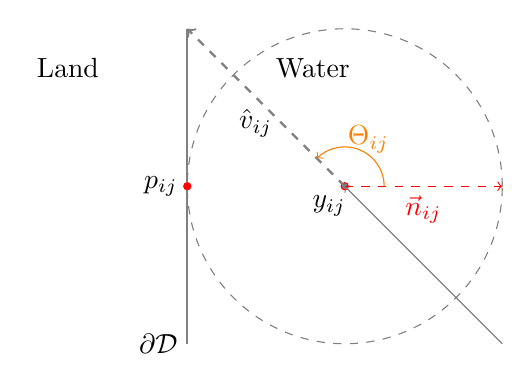
\begin{tikzpicture}
		%boundary
		\draw[gray, thick] (0,0) -- (0,4);
		%position
		\draw[red,fill=gray] (2,2) circle (.3ex);
		%nearest shore point
		\draw[red,fill=red] (0,2) circle (.3ex);
		%velocity
		\draw[->,gray] (4,0) -- (2,2);
		\draw[->,gray,dashed,thick] (2,2) coordinate (O) -- (0,4) coordinate (A);
		%normal vector
		\draw[->,red,dashed] (O) -- (4,2) coordinate (B);
		%trigonometric circle
		\draw[gray,dashed] (2,2) circle (2cm);
		%angle 
		\pic[draw=orange,->,angle eccentricity=1.2,angle radius=0.5cm] {angle=B--O--A};
		
		%nodes
		\node[left] at (-1,3.5) {Land};
		\node[right] at (1,3.5) {Water};
		\node[left] at (0,0) {$\partial \mathcal{D}$};
		\node[left] at (0,2) {$p_{ij}$};
		\node[left] at (1.2,2.8) {$\hat{v}_{ij}$};
		\node[below] at (1.8,2) {$y_{ij}$};
		\node[below,red] at (3,2) {$\vec{n}_{ij}$};
		\node[above,orange] at (2.3,2.3) {$\Theta_{ij}$};
	\end{tikzpicture}
	\caption{Example of nearest point on the shore and angle $\Theta$. $\partial D$ represents the boundary of the domain, $y_{ij}$ is the observed GPS position of narwhal $i$ at time $t_{ij}$.}
	\label{fig: illustration nearest shore points}
\end{figure}

The distance to the ship $D^{ship}$ (km) is defined as the distance between observed GPS locations of the ship and the narwhal. The values are comprised between $2.68$ and $63.8$ km.
Exposure to the ship for narwhal $i$ at time $t_{ij}$, denoted $E^{ship}_{ij}$, is defined as the inverse of the distance to the ship (in km) \citep{heide-jorgensen_behavioral_2021}. The covariate $E^{ship}$ is meant to be a proxy for sound exposure levels received by the narwhals. Reasonably, the closer the narwhal is to the ship, the louder is the sound, and thus the exposure is larger. 
$D^{ship}$ is only defined when the narwhal is in line of sight with the ship and exposures are set to $0$ when this is not this case. This implies that in the statistical model, the ship noise is only allowed to affect the narwhal when the ship is in line of sight, though it is likely that narwhals can perceive the disturbance even when they are not in line of sight with the sound source. This provides a conservative estimate of the effect of the noise exposure. Levels of the covariates $I^{shore}$ and $E^{ship}$ for each narwhal are displayed in Figure~\ref{fig: realexpthroughtime}.




\begin{figure}[ht!]
	\centering
	\begin{subfigure}{0.49\textwidth}
		\centering
		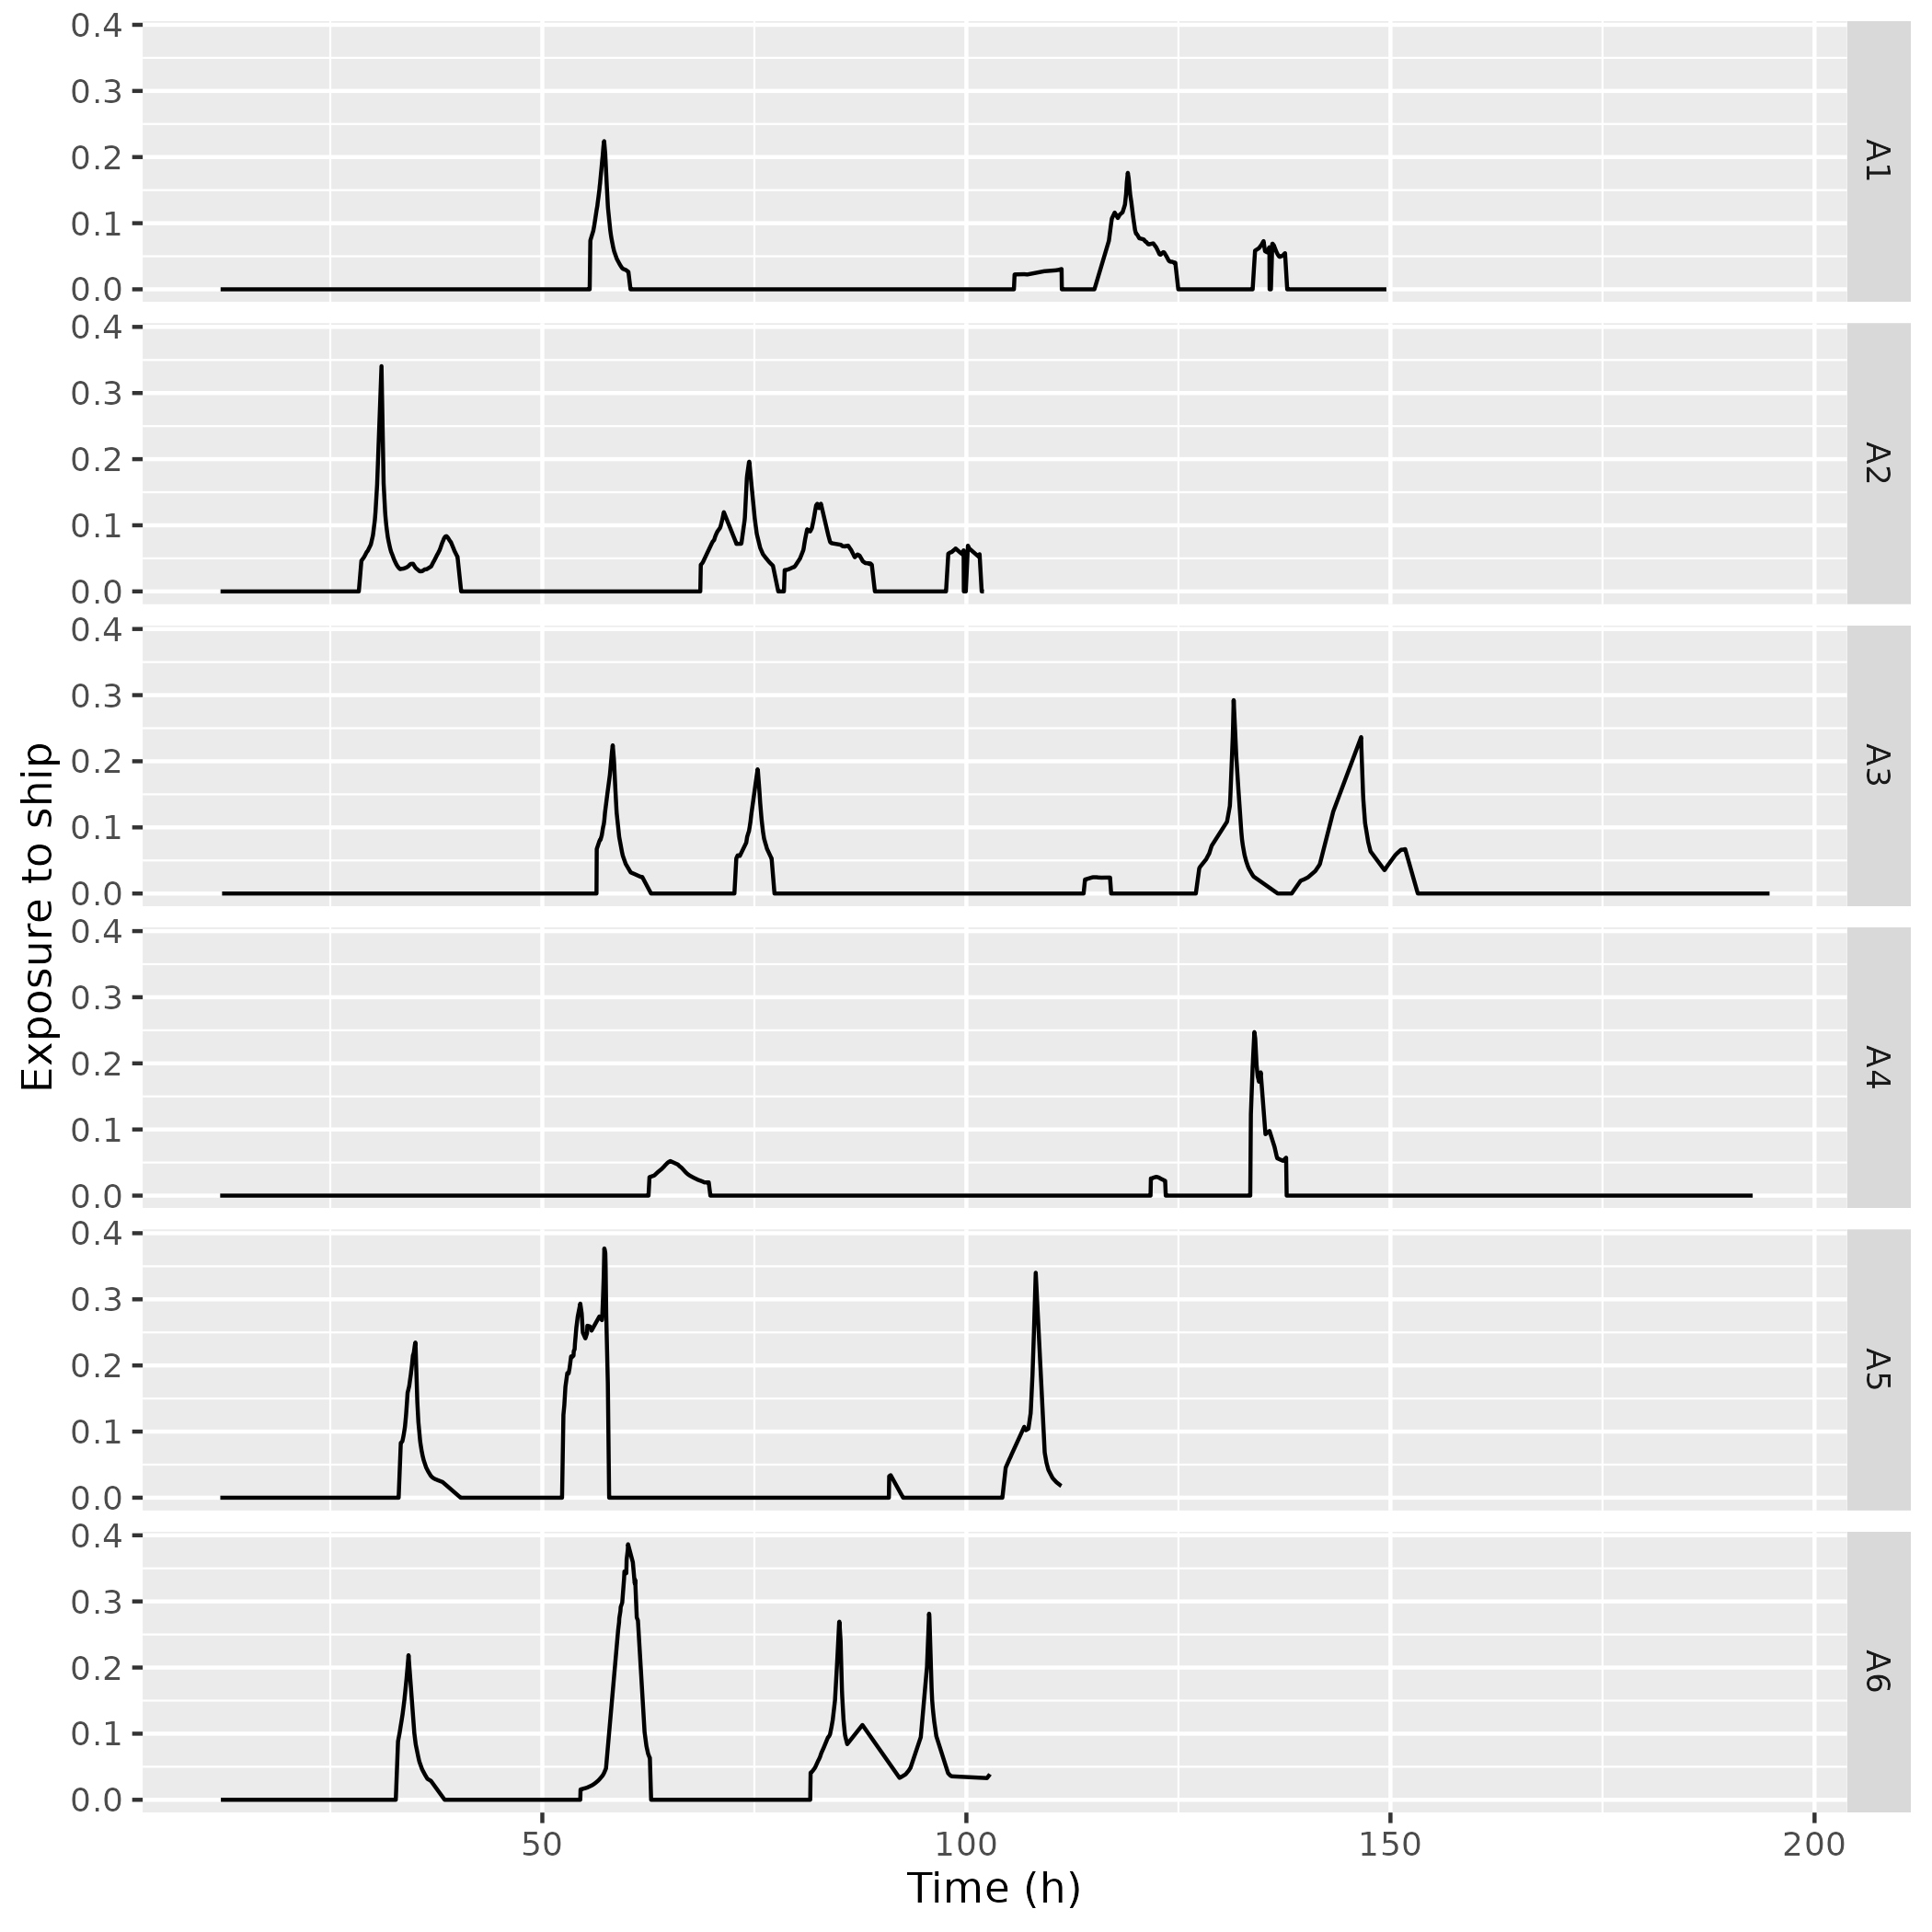
\includegraphics[scale=0.40]{images/data_exploration/realExpShip_through_time.png}
		\caption{}
	\end{subfigure}
	\begin{subfigure}{0.49\textwidth}
		\centering
		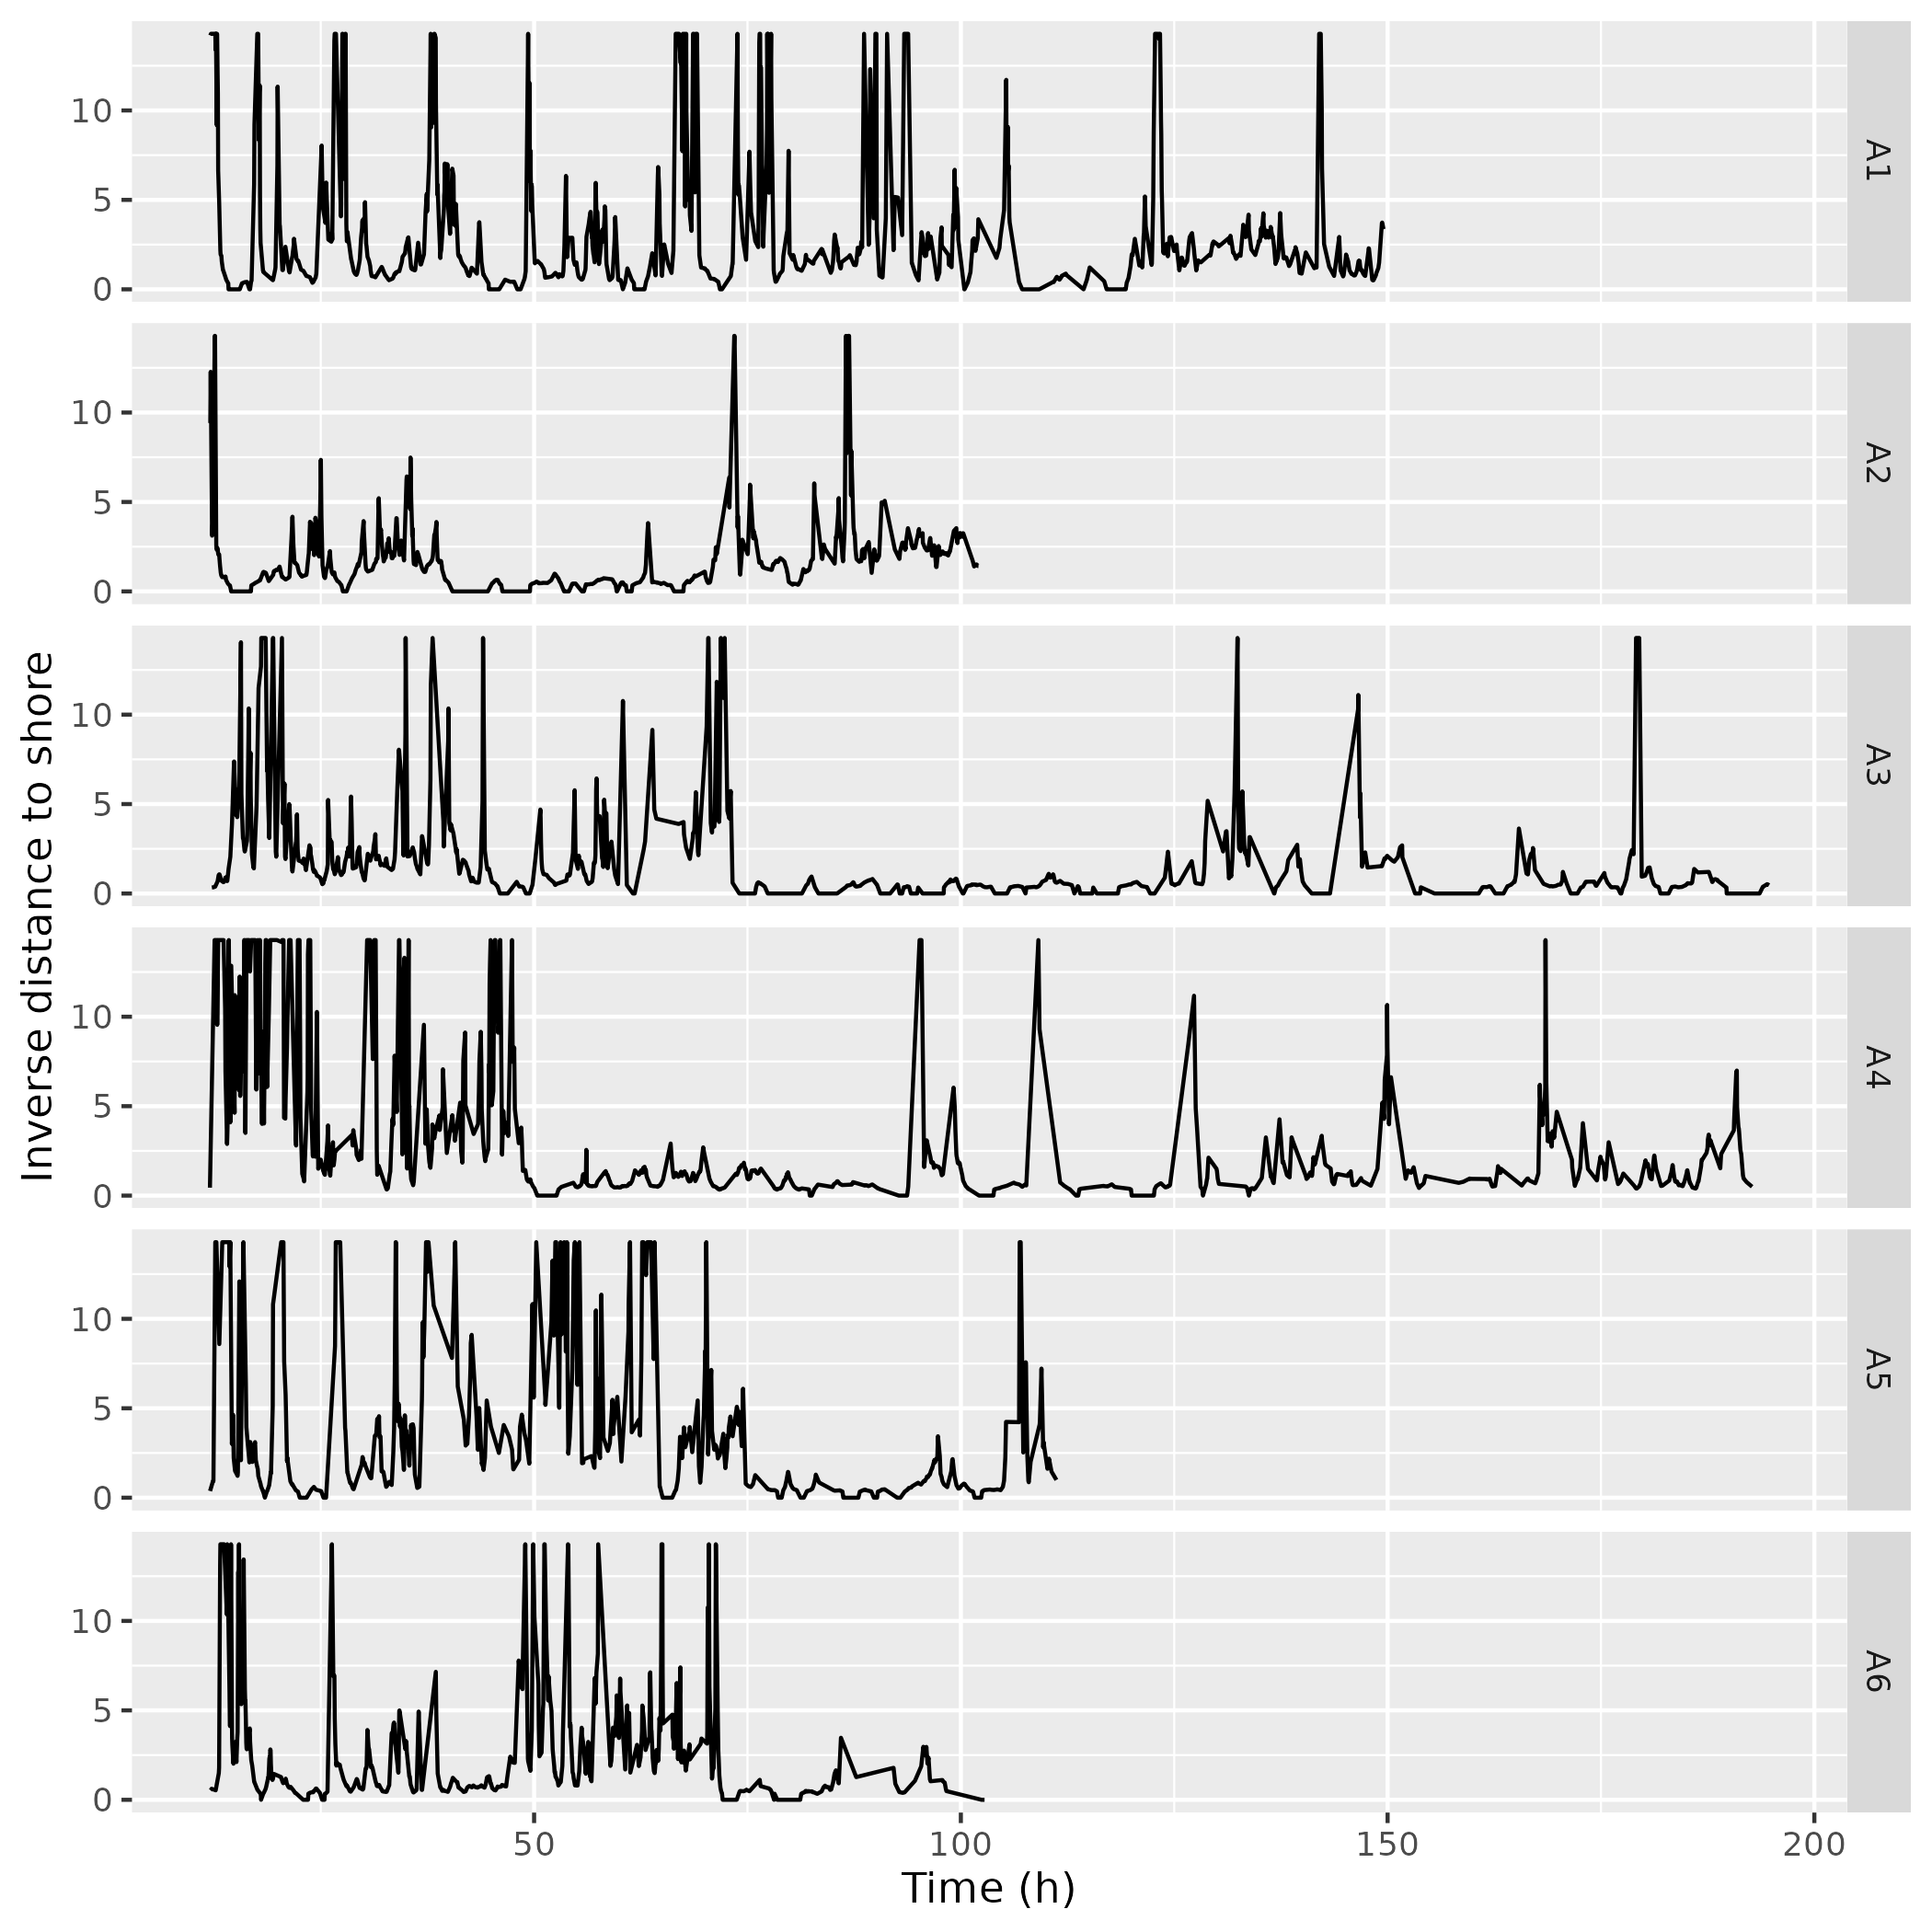
\includegraphics[scale=0.40]{images/data_exploration/realExpShore_through_time.png}
		\caption{}
	\end{subfigure}
	\caption{Covariates of exposure and distance to shore over time for each narwhal. Time 0 corresponds to 12 hours after tagging for each individual whale. (a) Exposure to the ship (in $km^{-1}$). (b) Inverse of the distance to the shore (in $km^{-1}$).}  
	\label{fig: realexpthroughtime}
\end{figure}



\section{Movement models within a constrained landscape}

The dynamics of the true positions of the narwhals is modelled by an SDE. First, we recall the standard rotational CVM, and then we extend it to include the effect of the distance to shore on the movement and constrain the position within a polygon.


\subsection{Standard Rotational Advective correlated velocity model (RACVM)}
\label{section: RACVM}
\mbox{}\\

Let $A=\begin{pmatrix} 
	\frac{1}{\tau} &&-\omega \\
	\omega && \frac{1}{\tau}
\end{pmatrix}$ and define

\begin{equation} \left\{
	\begin{array}{l}
		dX(t)=V(t)dt \\
		dV(t)=-A(V(t)-\mu)dt+\frac{2\nu}{\sqrt{\pi \tau}} dW(t) 
	\end{array}
	\right.
	\label{eq: RACVM equation}
\end{equation}
where $V(t)$ is the horizontal two-dimensional velocity at time $t$, $X(t)$ is the two-dimensional horizontal position, typically in longitude and latitude or in UTM coordinates, $W(t)$ is a two-dimensional brownian motion. Parameter $\tau$ is an autocorrelation time scale, $\nu$ controls the norm of the velocity and drives the random variability, $\mu=\begin{pmatrix} \mu_1 && \mu_2 \end{pmatrix}^\top$ is the long term velocity, and $\omega$ is an angular velocity that controls how fast the velocity vector rotates. The case $\omega=0$ corresponds to a standard CVM. In most applications, this standard model is satisfactory, but in case of tortuous movement, a non-zero value of $\omega$ is sometimes needed \citep{gurarie_correlated_2017,alt_correlation_1990,albertsen_generalizing_2018}. Moreover, whether or not to include a non-zero mean velocity parameter $\mu$ depends on the specific context of the study. Typically, it makes sense to have $\mu\neq (0,0)$ when examining migratory patterns or avoidance reactions from a fixed sound source. 
We refer to~\eqref{eq: RACVM equation} as "Rotational Correlated Velocity Model" (RCVM) when $\mu=(0,0)$, and "Rotational Advective Correlated Velocity Model" (RACVM) when $\mu \neq (0,0)$.\\

In this section, we derive the explicit transition density for the process $U=\begin{pmatrix} X && V \end{pmatrix}^\top$. Though this model is considered in several papers, we found no mention of the closed form formulas derived here. In \cite{gurarie_correlated_2017}, only the process $V$ is exhaustively studied, and the classical distributional results about this process are used for estimation and simulation purposes.
A more general formulation is considered by \cite{albertsen_generalizing_2018} in which the diffusion matrix is lower triangular with positive diagonal elements and two distinct autocorrelation parameters are considered in each direction allowing for anisotropic movement. In this case, \cite{albertsen_generalizing_2018} derives the Gaussian transition density of the velocity process, where the covariance matrix is expressed using a Kronecker sum. However, the formulas for the process $X$
are not provided, and the Euler scheme is employed to approximate the transition densities of $X$. This approach is generally sufficient when the animal’s positions are recorded at high frequency. Yet, for marine mammals such as narwhals that dive to great depths, GPS measurements are usually taken at irregular intervals, typically of several minutes, which can render the Euler scheme unsuitable. Additionally, incorporating covariates into the parameters of the SDE often requires approximating the transition density by assuming the covariates remain constant during each time step \citep{michelot_varying-coefficient_2021}. This results in two layers of approximation, possibly leading to unreliable estimation.\\

Here, we show that under the hypothesis of isotropic movement, with diagonal diffusion matrix as in~\eqref{eq: RACVM equation}, not only the velocity but also the position process has a closed form formula. This is stated in the following proposition.\\


\begin{proposition}
	Let $U(t)=\begin{pmatrix} X(t) && V(t) \end{pmatrix}^\top$ for $t \geq 0$ be the solution to \eqref{eq: RACVM equation}. Then the exact transition density of the Markov process $U$ is given by 
	\begin{equation}
		U(t+\Delta) \vert U(t)=u \sim \mathcal{N}\left( T(\Delta) u +B(\Delta)\mu, Q(\Delta)\right) \mbox{ for all } \Delta>0 \mbox{ and } u \in \R^4
		\label{eq: X V distribution}
	\end{equation}
	where \begin{equation}
		T(\Delta)=\begin{pmatrix} I_2 && A^{-1}(I_2-\exp(-A\Delta)) \\
			0_2 && \exp(-A\Delta) \end{pmatrix} \mbox{, } B(\Delta)=\begin{pmatrix}
			\Delta I_2 -A^{-1}(I_2-\exp(-A\Delta))\\
			I_2-\exp(-A\Delta)\end{pmatrix}
		\label{eq: link matrices}
	\end{equation}
	and the covariance block matrix is given by
	\begin{equation}
		Q(\Delta)=\begin{pmatrix}
			q_1(\Delta)I_2 && \Gamma(\Delta) \\
			\Gamma(\Delta)^\top && q_2(\Delta)I_2
		\end{pmatrix}
		\label{eq: covariance matrix}
	\end{equation}
	with 
	\begin{equation*}q_1(\Delta)=\frac{\sigma^2}{C}\left( \Delta-2 \frac{\omega \sin(\omega \Delta)-\frac{1}{\tau} \cos(\omega \Delta)}{C} \exp\left( -\frac{\Delta}{\tau} \right) +\frac{\tau}{2} \left( \frac{\omega^2-\frac{3}{\tau^2}}{C}-\exp\left( -\frac{2\Delta}{\tau}\right)\right) \right)
	\end{equation*}
	
	\begin{equation*}
		q_2(\Delta)=\frac{2\nu^2}{\pi}\left(1-e^{-\frac{2 \Delta}{\tau}}\right)
	\end{equation*}
	\begin{equation*}\Gamma(\Delta)=\begin{pmatrix} \gamma_1 && \gamma_2 \\
			-\gamma_2 && \gamma_1\end{pmatrix}
	\end{equation*}
	where
	\begin{equation*}\gamma_1=\frac{\sigma^2}{2 C } \times \left( 1+\exp\left( -\frac{2\Delta}{\tau}\right)-2\exp\left( -\frac{\Delta}{\tau}\right) \cos(\omega\Delta)\right)
	\end{equation*}
	\begin{equation*}\gamma_2=\frac{\sigma^2}{C} \times\left( \exp\left( -\frac{\Delta}{\tau}\right) \sin(\omega \Delta)-\frac{\omega \tau}{2} \left(1-\exp\left( -2 \frac{\Delta}{\tau}\right) \right)\right)
	\end{equation*}
	and we denoted $C=\frac{1}{\tau^2}+\omega^2$ and $\sigma=\frac{2\nu}{\sqrt{\pi \tau}}$.
	\label{prop: transition density}
\end{proposition}

The formulas derived in \citep{johnson_continuous_2008} are a corollary of Proposition~\ref{prop: transition density}, obtained with $\omega=0$. The proof of this proposition is detailed in Appendix.

Equation~\eqref{eq: covariance matrix} shows that the two components of the location and velocity processes are independent.
Note that $\exp(-A\Delta)=e^{\frac{-\Delta}{\tau}} \begin{pmatrix} \cos(\omega \Delta) && \sin(\omega \Delta) \\ -\sin(\omega \Delta) && \cos(\omega \Delta) \end{pmatrix}$ is a weighted rotation matrix of angle $-\omega \Delta$.
Intuitively, ~\eqref{eq: X V distribution} means that the next velocity $V(t+\Delta)$ is a weighted mean of the long term mean velocity $\mu$ and the previous velocity $V(t)$ rotated by an angle $-\omega \Delta$.\\


For locomotion under spatial constraints, we hypothesize that an increase in tortuosity is a sign of avoiding the boundary and adapting the heading to the spatial constraint. We use this to define a constrained version of the standard RCVM.

\subsection{Constrained rotational correlated velocity model}
\label{section: CRCVM}

We propose a new RCVM that relies on the tortuosity parameter, or angular velocity $\omega$, to describe how the animals turn in reaction to the shore. 
To do so, we consider $\omega$ as a smooth function both of the distance to the shore $D^{shore}$ and the angle between the velocity vector and the shore normal vector $\Theta$. 
We write $\mathcal{D} \subset \R^2$ for the polygon defining the domain of the process $X$. The new formulation of the equation is 
\begin{equation} \left\{
	\begin{array}{l}
		dX(t)=V(t) dt \\
		dV(t)=-A(X(t),V(t))V(t)dt+\frac{2\nu}{\sqrt{\pi \tau}} dW(t) 
		
	\end{array}
	\right.
	\label{eq: CRCVM equation}
\end{equation}
with 
\begin{equation} 
	A(X(t),V(t))=\begin{pmatrix} 
		\frac{1}{\tau} && -\omega(X(t),V(t)) \\
		\omega(X(t),V(t)) && \frac{1}{\tau}
	\end{pmatrix}
	\label{eq: CRCVM matrix A}
\end{equation}
where $\omega(X(t),V(t))=f_{\omega}(D^{shore}(t),\Theta(t))$ with  $f_{\omega}$ a smooth function from $\R^{+} \times [-\pi,\pi]$ to $\R$. In the sequel, such models will be refered to as Constrained Rotational Correlated Velocity Models (CRCVM).\\

To induce a rotation when the animal is close to the boundary and heading in the direction of the shore,
the following assumptions must guide the shape of $f_{\omega}$:
\begin{itemize}
	\item[1)] for a distance to the shore lower than some threshold, $f_{\omega}(D^{shore},\cdot)$ should be positive and increasing on $]\frac{\pi}{2},\pi[$, 
	\item[2)] for a distance to shore  lower than some threshold, $f_{\omega}(D^{shore},\cdot)$ should be negative and decreasing on $]-\pi,-\frac{\pi}{2}[$,
	\item[3)] as distance to shore decreases, the magnitude of the functions  $f_{\omega}(D^{shore},\cdot)$ on $]\frac{\pi}{2},\pi[$  and $]-\pi,-\frac{\pi}{2}[$ should increase.
\end{itemize} 


We start by proposing a parametric model for the function $f_{\omega}$ and then discuss a non-parametric representation. For $\Theta \in [-\pi,\pi]$ and $D^{shore} \geq0$, we define $f_{\omega}$ as follows

\begin{equation}
	\label{eq: smooth omega}
	f_{\omega}(\Theta,D^{shore})=\frac{\omega_0}{2}\left(\tanh(\lambda(\Theta+\theta^{*}))+\tanh(\lambda(\Theta-\theta^{*})))\right)\times \exp\left(-\kappa \times \left(\frac{D^{shore}}{D_0}\right)^2\right)
\end{equation}
for some $D_0>0$, $\kappa>0$, $\omega_0 \in \R$, $\lambda>0$, $\theta^* \in [0,\pi]$.
The parameter $\omega_0$ controls the magnitude of the angular velocity, $D_0$ controls the distance at which the velocity starts to rotate to avoid the boundary, $\lambda$ and $\kappa$ control the steepness of the curves in each dimension, and $\theta^*$ is chosen so that the rotation starts when the angle $\Theta$ gets close to $\frac{\pi}{2}$ or $-\frac{\pi}{2}$. \\

This parametrization of $\omega$ is motivated by the observations above, and do not pretend to be optimal. 
Any smooth function, including~\eqref{eq: smooth omega}, could be approximated by a finite number of weighted spline basis functions of the form

\[f_\omega(\Theta,D^{shore})=\sum_{k=1}^L \omega_k \psi_k(\Theta,D^{shore})\]
The $\psi_k, k=1, \ldots, L$ can be constructed in several ways based on thin plate regression splines, or on the tensor product of any univariate spline basis. The coefficients $\omega_k$ control the contribution of each basis function to the final shape of the smooth function \citep{wood_generalized_2017}. Figure~\ref{fig: combinedperspplots}  shows function~\eqref{eq: smooth omega} in the top, along with a smooth function $f_{\omega}$ obtained as a combination of $L=9$ cubic spline basis functions approximating~\eqref{eq: smooth omega} in the bottom plots. 

\begin{figure}[ht!]
	\centering
	\begin{subfigure}{0.48\textwidth}
		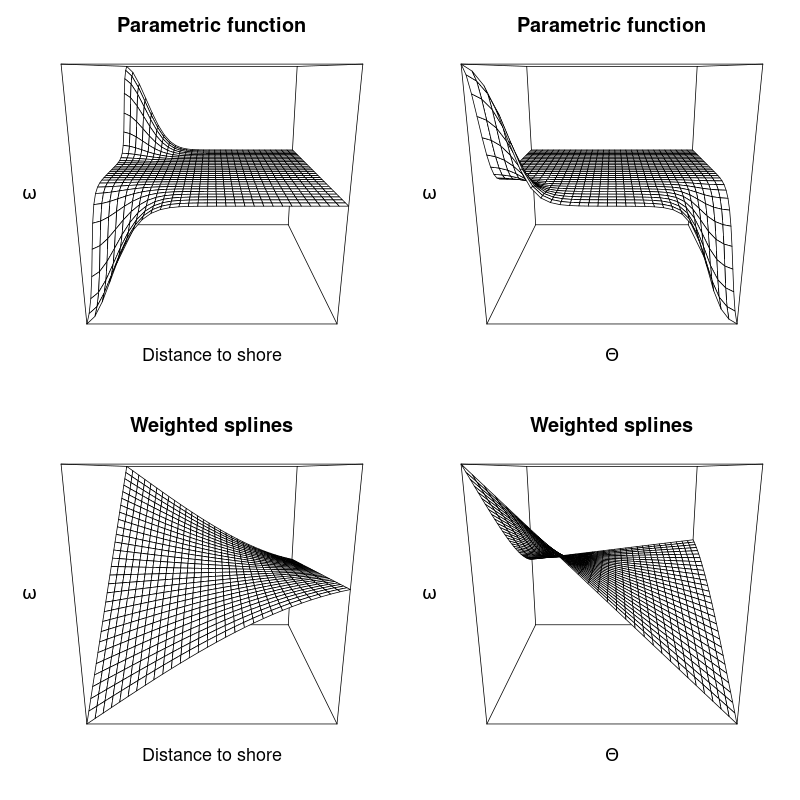
\includegraphics[scale=0.25]{images/crcvm/combined_persp_plots.png}
		\caption{}
		\label{fig: combinedperspplots}
	\end{subfigure}
	\begin{subfigure}{0.48\textwidth}
		\centering
		\raisebox{0.5cm}{
			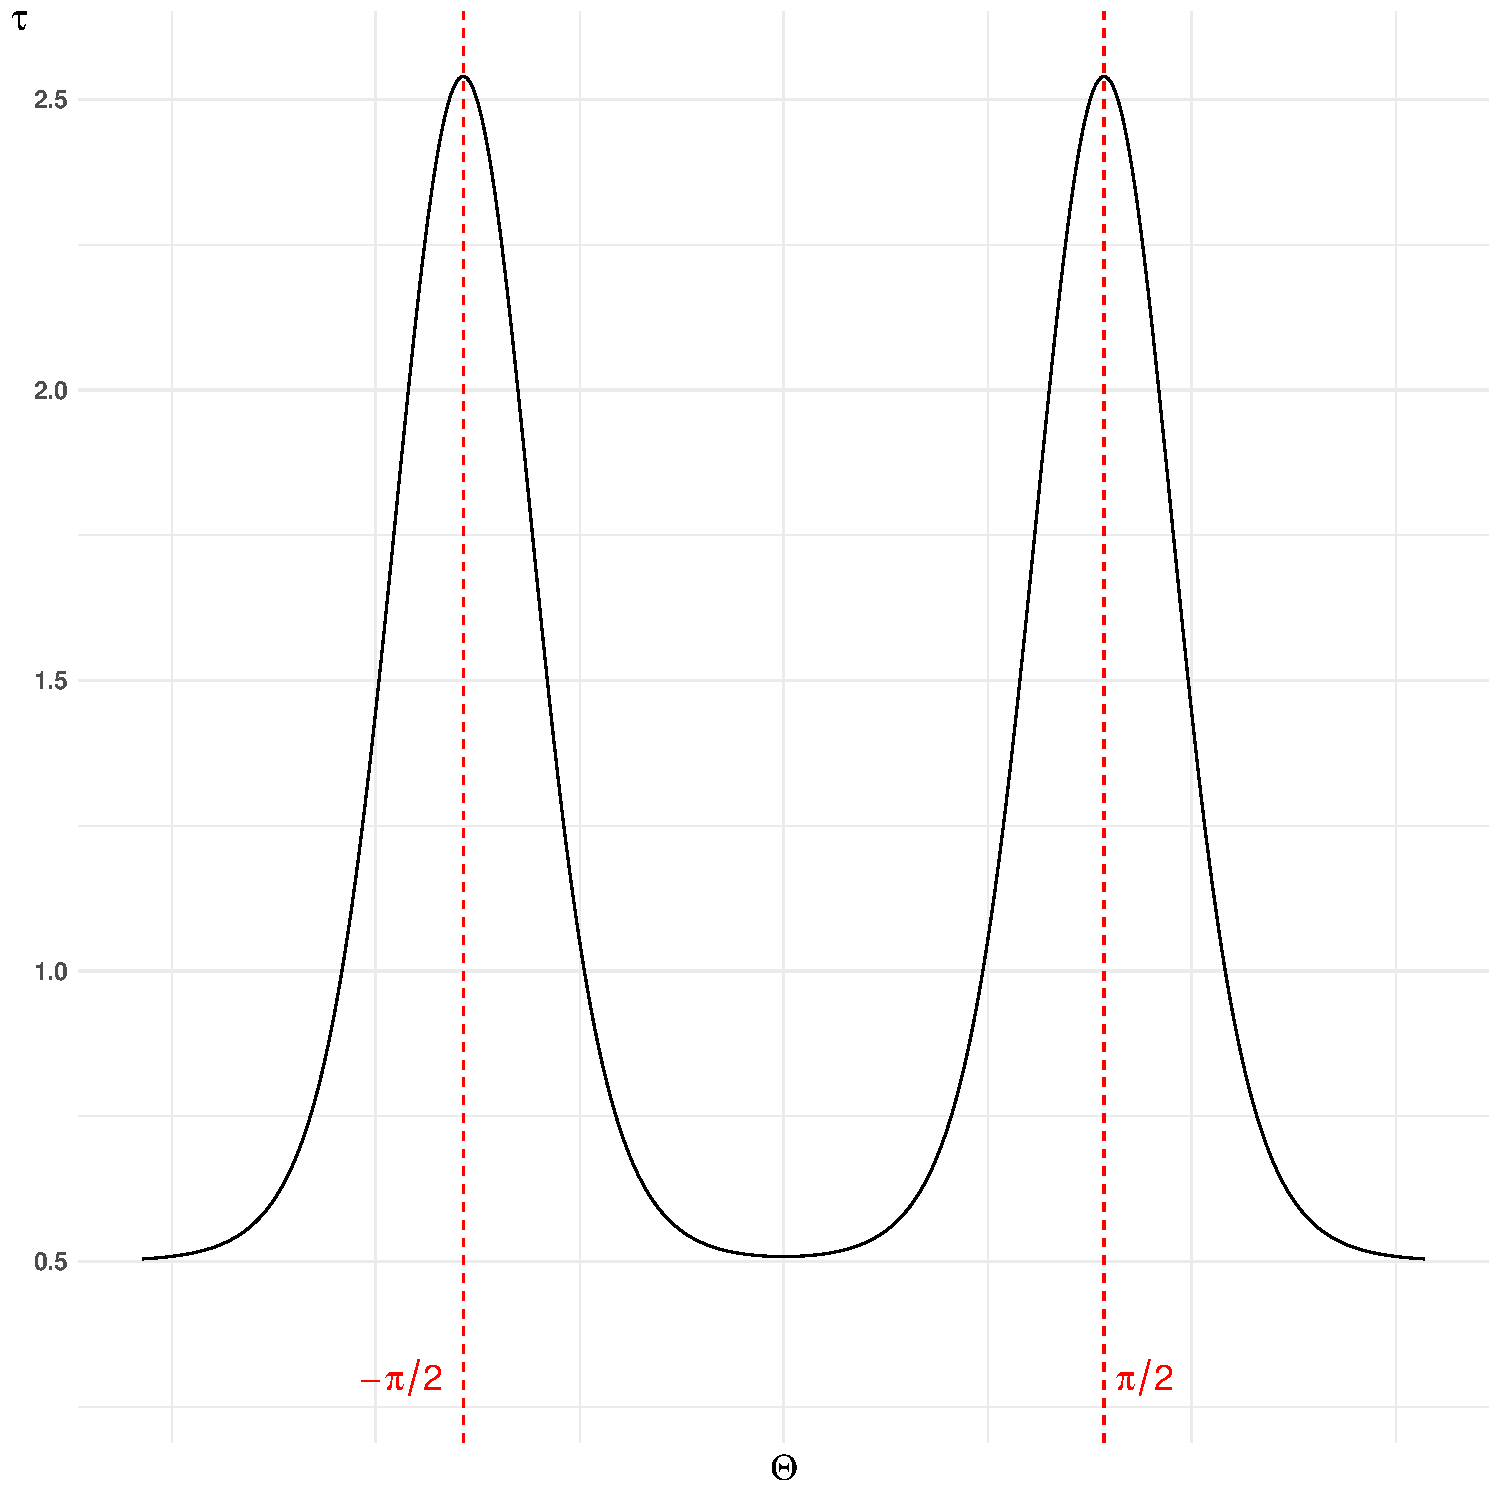
\includegraphics[scale=0.25]{images/crcvm/smooth_tau_bump.pdf}
		}
		\caption{}
		\label{fig: smoothtau}
	\end{subfigure}
\caption{(a) Examples of smooth functions $f_{\omega}$. Angular velocity $\omega$ increases as $\Theta$ approaches $\pm\pi$, and decreases with increasing distance to the shore.  Top: Two views of the smooth function $f_{\omega}$ defined by~\eqref{eq: smooth omega} with values $D_0=0.3$ km, $\kappa=0.2$, $\lambda=2$, $\omega_0=\frac{\pi}{2}$ rad/min. Bottom: Two views of a smooth function $f_{\omega}$ obtained by combining nine bivariate cubic spline basis functions approximating~\eqref{eq: smooth omega}. (b) Example of a smooth parameter $\tau$ to get persistent trajectories along the shore. The function used is $\tau_0+\frac{\tau_1-\tau_0}{2}\times \left(\tanh(\frac{\Theta+\pi/2+\varepsilon}{\alpha})-\tanh(\frac{\Theta+\pi/2-\varepsilon}{\alpha})+\tanh(\frac{\Theta-\pi/2+\varepsilon}{\alpha})-\tanh(\frac{\Theta-\pi/2-\varepsilon}{\alpha})\right)$ for some parameters $\tau_0$, $\tau_1$, $\varepsilon$, $\alpha$.}
	
\end{figure}

Model~\eqref{eq: CRCVM equation} is flexible, and different species-specific behaviours can be described. Function $f_{\omega}$ controls at which distance the animal will turn away from the shore, and how fast it will turn.  Specific constraints on the smooth function $f_{\omega}$ can be set from biological knowledge about the species in question. 

The tendency of an animal to move along the boundary of its spatial domain can be captured by the parameter $\tau$, as more persistent movement when the angle $\theta$ is close to $\pm\frac{\pi}{2}$ would induce such behavior. More precisely, to model persistent movement along the shoreline, we modify~\eqref{eq: CRCVM matrix A} by expressing $\tau$ as a smooth function:
\[\tau(X(t),V(t))=f_{\tau}(\Theta(t))\] with $f_{\tau}:[-\pi,\pi] \longrightarrow \R$.
The function $f_{\tau}$ is defined such that it reaches local maximas in $\Theta=\pm\frac{\pi}{2}$, which represents movement along the boundary of the domain. An example of such a function is given in Figure~\ref{fig: smoothtau}. However, for simplicity we will assume $\tau$ constant in our analysis of the data.\\


Solving explicitly~\eqref{eq: CRCVM equation} is out of reach due to the non-linearity induced by the distance to the shore and the angle $\Theta$. But it is possible to get an approximate solution. We choose a time step $\Delta$ and approximate $D^{shore}$ and $\Theta$ by piecewise constant functions on each time step. We then use the formulas of Section~\ref{section: RACVM} to simulate the process and get the next position from the approximate transition densities. Sampled trajectories obtained within circular, rectangular and fjord domains for different smooth functions $f_{\omega}$ and $f_{\tau}$ are shown in Figure~\ref{fig: crcvm examples}. Depending on the smooth functions $f_{\omega}$ and $f_{\tau}$, the trajectories near the boundary have different characteristics. The trajectories labelled "persistent" tend to keep the same direction along the boundary, while the trajectories labelled standard turn whenever they are about to hit the boundary, and behave like an unconstrained CVM with $\omega=0$ otherwise.  The trajectories labelled "tortuous" also turn when going toward the shore, but keep turning when leaving the shore.\\

\begin{figure}[ht!]
	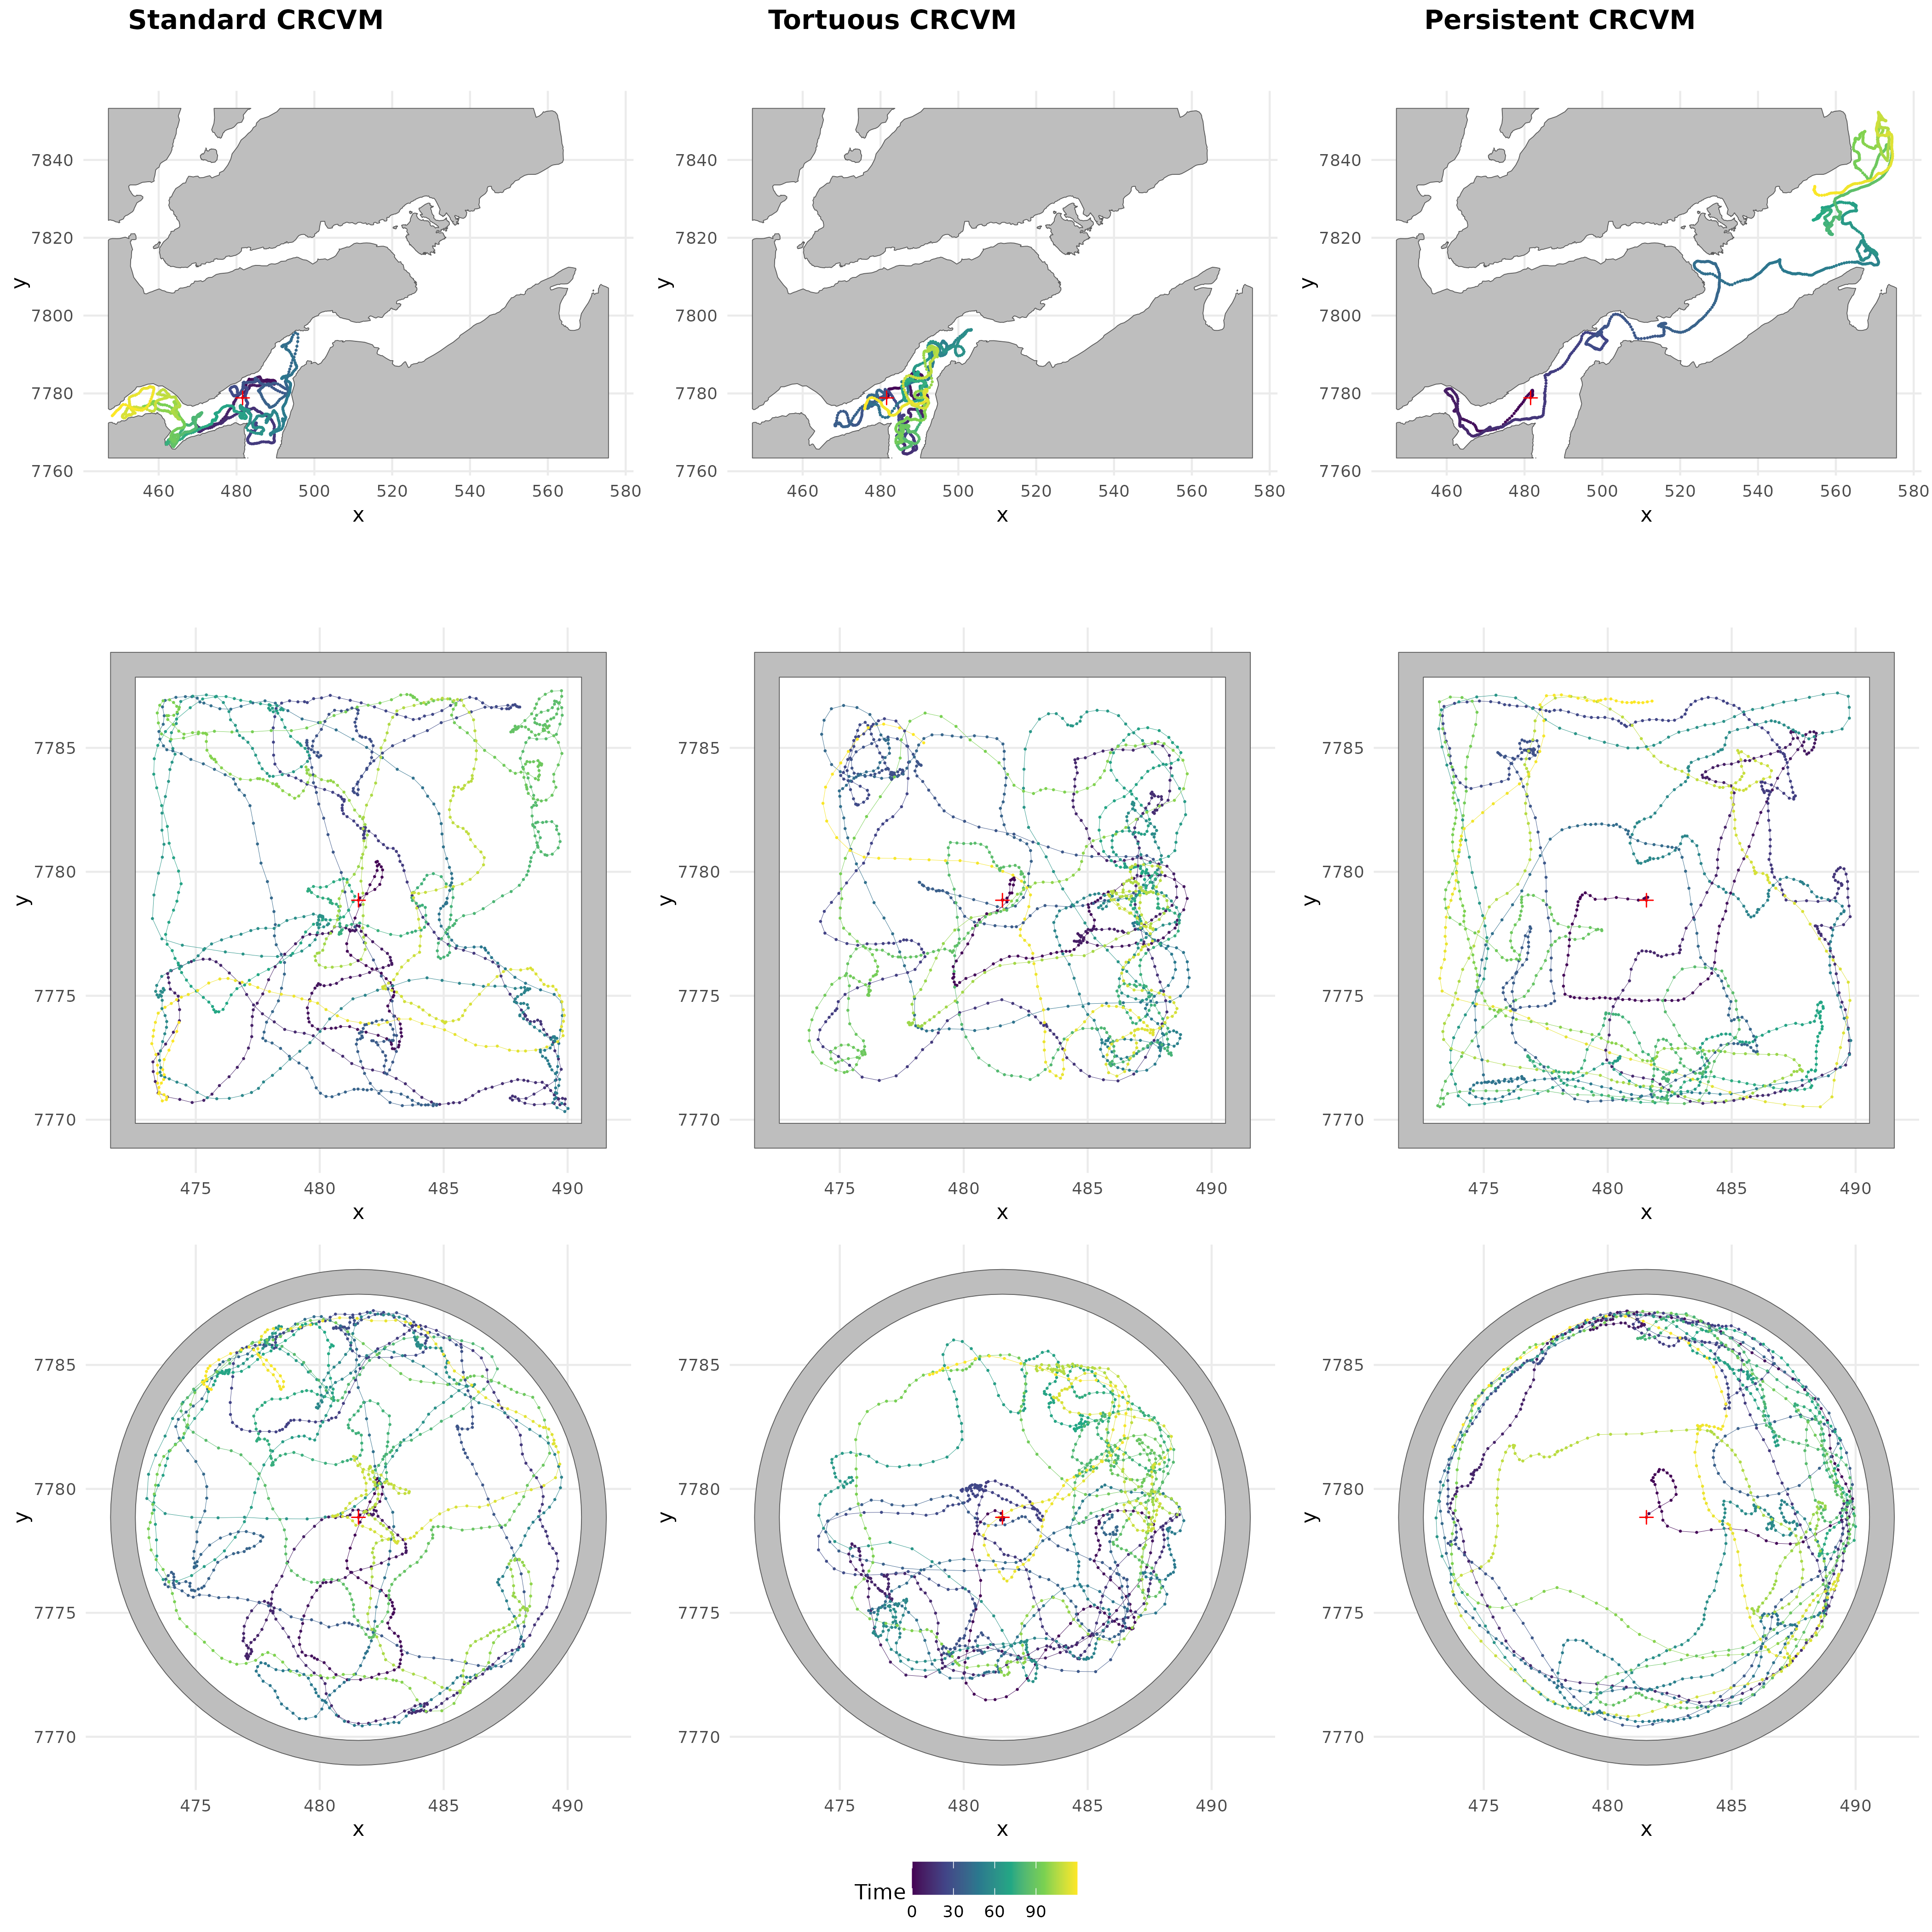
\includegraphics[scale=0.4]{images/crcvm/final_combined_plot.png}

	\caption{Five days trajectories with time step $\Delta=5$ min within circular (bottom), rectangular (middle) and fjords (top) domains. Plots labelled "Persistent CRCVM" and "Standard CRCVM" have the same smooth parameter $\omega$ defined by~\eqref{eq: smooth omega}, whereas the persistent trajectory has a smooth varying parameter $\tau$ as in Figure~\ref{fig: smoothtau}. The standard trajectory has a constant $\tau =1$h. Trajectories labelled "tortuous" are obtained from a constant $\tau=1$h and a smooth parameter $\omega$ defined with spline basis functions as in Figures~\ref{fig: combinedperspplots}. All trajectories have constant velocity parameter $\nu=4$km/h.}
 \label{fig: crcvm examples}
\end{figure}



While we have not established formal theoretical conditions for the function $f_{\omega}$ to guarantee constrained motion,   illustrative examples demonstrate how smooth, interpretable functions can produce constrained trajectories for the process $X$. A critical parameter in this model is the spatial scale of the rotational movement, defined as $\rho=\frac{\nu}{\vert \omega \vert}$, representing the diameter of rotation. To prevent the animal from hitting the boundary, $\rho$ should remain smaller than $D^{shore}$.\\


We will use the CRCVM \eqref{eq: CRCVM equation} allowing $\omega$ to vary to analyze narwhals trajectories while considering spatial constraints, whereas we keep $\tau$ fixed. In section~\ref{section: simulation constrained motion}, we show that a smooth function $f_{\omega}$ depending on $D^{shore}$ and $\Theta$ can be estimated from discrete time obsevations of the process $X$.




\section{Inference of the sound exposure effect}

To analyse potential perturbations in the locomotion of the narwhals due to sound exposure, we formulate a statistical mixed effect model for the parameters of the CRCVM, and discretise~\eqref{eq: X V distribution} to get an approximate state space model for inference with the Kalman filter.


\subsection{Mixed effect CRCVM model for  shore influence and sound exposure}
\label{subsection: ship exposure effect}


First a baseline model is fitted only on the data before exposure, to get an estimate of natural behavior, when the narwhals are not exposed to the ship and airgun sounds. Then, a response model is fitted on the data during exposure to test whether the estimated smooth parameters deviate significantly from the baseline values. We present here the baseline and response models.\\

For the baseline model, only the effect of the shore is included through the covariates $I^{shore}$ and $\Theta$. For each narwhal $i \in \{1, \cdots, N\}$ and each time $j\in\{1, \cdots, n_{i,pre}\}$, $y_{ij}$ is an observation with measurement error of position $X_{ij}$:

\begin{equation}
	y_{ij}=X_{ij}+\varepsilon_{ij} \quad 
	\varepsilon_{ij} \underset{i.i.d}{\sim} \mathcal{N}(0,\sigma_{obs}^2)  
	\label{eq: baseline observations}
\end{equation}
%The process  $V_{ij}$ is  unobserved. 
The standard deviation $\sigma_{obs}$ represents GPS measurement errors variability. The assumption of i.i.d. Gaussian measurement errors is a simplified model of actual GPS measurement errors. In practice, the accuracy of GPS positions is influenced by the number of satellites processing the GPS signal—more satellites generally result in more accurate positions. Furthermore, the error can differ between the $x$ and $y$ directions. For a comprehensive study on Fastloc-GPS measurement errors, we refer to \citep{wensveen_path_2015}. It is often more appropriate to use a distribution with heavier tails, such as the Student's $t$-distribution, to model measurement error. However, this introduces additional complexity to the inference process, as a standard linear Kalman filter cannot be directly applied in such cases. Since the Student's $t$-distribution approaches a Gaussian distribution as its degrees of freedom increase, the Gaussian distribution is considered a reasonable trade-off between simplicity and suitability.\\

%We denote $\tau_i$, $\nu_i$, $\omega_i$ the parameters of the CRCVM for narwhal $i$. 
The latent processes $X_i$ and $V_i$ solve 


\begin{equation}  %\forall i \in \{1,\cdots,N\}, \quad 
	\left\{
	\begin{array}{l}
		dX_i(t)=V_i(t)dt  \\
		dV_i(t)=-\begin{pmatrix} 
			\frac{1}{\tau_i} && -\omega_i(t) \\
			\omega_i(t) && \frac{1}{\tau_i}
		\end{pmatrix}V_i(t)dt+\frac{2\nu_i}{\sqrt{\pi \tau_i}} dW(t) \\
	\end{array}
	\right.
	\label{eq:baseline latent processes}
\end{equation}
%
where $\tau_i$, $\nu_i$ are individual parameters   to account for variability between narwhals:
%
\begin{equation}   
	%\begin{array}{l}
	\begin{pmatrix}	\log(\tau_i)\\ \log(\nu_i) \end{pmatrix}
	= \begin{pmatrix}\log(\tau_0)\\ \log(\nu_0) \end{pmatrix}
	+
	\begin{pmatrix} b_{\tau,i}\\  b_{\nu,i}  \end{pmatrix}
	\quad \mbox{ with } \quad
	\begin{pmatrix} b_{\tau,i} \\ b_{\nu,i} \end{pmatrix} \underset{i.i.d}{\sim} \mathcal{N}\left(0,\begin{pmatrix} \sigma_{\tau}^2 && 0 \\ 0 && \sigma_{\nu}^2 \end{pmatrix}\right) 
	%\end{array}
	\label{eq:baseline random effects}
\end{equation}

Since $\tau$ and $\nu$ are positive, a log link function is used for these parameters. The coefficients $\log(\tau_{0})$, $\log(\nu_{0})$ are population intercepts and $b_{\tau,i}$, $b_{\nu,i}$
are the individual random effects. \\

Finally, as discussed in Section \ref{section: CRCVM}, the angular velocity function of individual $i$, $\omega_i$, is expressed as a smooth function of $\Theta$ and $I^{shore}$ through splines: 
%
\begin{equation} 
	\omega_i(t)=\omega_{0}+\sum_{k=1}^{L} \omega_{k} \psi_k(I_i^{shore}(t),\Theta_i(t))
	\label{eq: baseline splines}
\end{equation}


Since the two covariates are not on the same scale (one is in $rad$ while the other is in $km^{-1}$), tensor splines are more appropriate than thin plate regression splines.
The functions $\psi_k$ in equation~\eqref{eq: baseline splines} are the bivariate basis functions constructed from univariate cubic spline basis functions. We refer to \citep{wood_generalized_2017} section $4.
1.8$ for the construction of tensor splines basis functions. The splines degree of freedom is $L=q_E \times q_{\Theta}$ and the number of knots in the splines are $q_E-1$ and $q_{\Theta}-1$ for the covariates $I_{shore}$ and $\Theta$, respectively.\\


The response model is then designed to assess a deviation from the baseline model due to exposure to the ship. The observations are supposed to have the same measurement errors as the baseline. For $i \in \{1, \ldots, N\}$ and $j \in \{n_{i,pre}+1,\cdots,n_{i,post}\}$, we have

\begin{equation}  		y_{ij}=X_{ij}+\varepsilon_{ij}, \quad 		\varepsilon_{ij} \underset{i.i.d}{\sim} \mathcal{N}(0,\sigma_{obs}^2) 
	\label{eq: response observations}
\end{equation}

Then we add a dependency on the covariate $E_{ship}$ in the parameters $\tau_i$ and $\nu_i$: 
\begin{equation}    
	\begin{array}{l}
		\log(\tau_{i}(t))=\log(\tau_{0})+\alpha_{\tau} E^{ship}_i(t)+b_{\tau,i} \\
		\log(\nu_{i}(t))=\log(\nu_{0}) +  \alpha_{\nu} E^{ship}_i(t) +b_{\nu,i}  \\
	\end{array}
	\label{eq:response loglinear model}
\end{equation}


The intercepts $\log(\tau_0)$, $\log(\nu_0)$ and the smooth $\omega$ from the baseline model enter as offsets in the response model.
Thus, only the coefficients $\alpha_{\tau}$ and $\alpha_{\nu}$ are estimated from the data during exposure. These parameters control the deviation of $\tau_i$ and $\nu_i$ from their baseline values $\tau_0$ and $\nu_0$ as a function of the distance to the ship. Coefficients $\alpha_{\tau}$ and $\alpha_{\nu}$ significantly deviating from $0$ indicate an effect of the sound exposure on the narwhals horizontal motion.




\subsection{Linear Gaussian state-space model}
\label{section: state space model}
In the baseline statistical model \eqref{eq:baseline latent processes}, we make the approximation suggested in \citep{michelot_varying-coefficient_2021} that the function $\omega_i$ is constant on each time step $[t_{ij},t_{i,j+1}]$, equal to its value at time $t_{ij}$, that is 
\[\forall t \in [t_{ij},t_{i,j+1}], \quad \omega_{i}(t) \simeq \omega(t_{ij})=\omega_{0}+\sum_{k=1}^{L} \omega_{k} \psi_k(I_{ij}^{shore},\Theta_{ij}).\]
We write %$\Delta_{ij}=t_{i,j+1}-t_{ij}$, $V_{ij}=V(t_{ij})$, $X_{ij}=X(t_{ij})$, 
$\omega_{ij}=\omega(t_{ij})$, $A_{ij}=\begin{pmatrix} 
	\frac{1}{\tau_{i}} && -\omega_{ij} \\
	\omega_{ij} && \frac{1}{\tau_{i}}
\end{pmatrix}$ and $U_{ij}=\begin{pmatrix} X_{ij,1}  && X_{ij,2} && V_{ij,1} && V_{ij,2}\end{pmatrix}^\top$. % where $\log(\tau_i)=\log(\tau_0)+b_{\tau}^{(i)}$ and $\log(\nu_i)=\log(\nu_0)+b_{\nu}^{(i)}$.
%
We use the exact formulas from Proposition \ref{prop: transition density} to obtain the state-space matrix equations for $i\in\{1,\ldots, N\}$, and $j\in\{1, \ldots, n_{i,pre}\}$:%.
%Discretisation of~\eqref{eq: X V distribution} gives the following system:

\begin{equation}
	\begin{array}{l}
		y_{ij}=ZU_{ij}+\varepsilon_{ij},  \quad 
		\varepsilon_{ij} \underset{i.i.d}{\sim} \mathcal{N}(0,\sigma_{obs}^2) \\
		U_{i,j+1}=T_{ij}\,U_{ij} + \eta_{ij}, \quad 
		\eta_{ij} \sim \mathcal{N}(0,Q_{ij})
	\end{array}
	\label{eq: RACVM state space}
\end{equation}
where $Z=\begin{pmatrix} I_2 && 0_{2,2}\end{pmatrix}$, the link matrix $T_{ij}$ is computed according to~\eqref{eq: link matrices} and the covariance matrix $Q_{ij}$ is computed according to~\eqref{eq: covariance matrix}.
\\
A linear Gaussian state-space model is obtained similarly for the response model. Estimation with $\texttt{smoothSDE}$ relies on this state-space formulation.
The complete likelihood is computed from the observations $y_{ij}$ as a by-product of the Kalman filter algorithm \citep{michelot_varying-coefficient_2021}.
Laplace's approximation of the integral of this complete likelihood over the random effects is computed using the \texttt{R} package \texttt{TMB}  and optimization is performed via the \texttt{optim} function in $\texttt{R}$ with the BFGS gradient method, with the gradient being calculated by automatic differenciation. We refer to \citep{kristensen_tmb_2016} for more details about the derivation of the multidimensional Laplace's approximation and the gradient computations. We refer to \cite[section 6.6]{wood_generalized_2017} for the specification of the mixed effect model and the regularization terms that are based on a wiggliness measure involving Gaussian priors for the spline coefficients $\omega_k$, $k \in \{1,\cdots,L\}$. \\
This method is already implemented for the CVM ($\omega=0$) in \texttt{smoothSDE}. Here, we extend this inference method to the more general model~\eqref{eq: CRCVM equation} and use it for estimation of the baseline and the response models.




\section{Simulation study for the baseline model}
\label{section: simulation constrained motion}
To test the estimator of the constrained model for our application, we simulate CRCVM trajectories in the Scoresby Sound fjord system. We consider observations of a baseline model as described in Section~\ref{subsection: ship exposure effect}. We set $L=9$ degrees of freedom for the bivariate splines in the parameter $\omega$ and  we place the knots evenly between $-\pi$ and $\pi$ for the covariate $\Theta$, and between $1$ and $5$ km for $D^{shore}$. The values of the spline coefficients are chosen to get a process that turns fast enough to meet the spatial constraints. We fix $\tau_0=1.5$ h and $\nu_0=4$ km/h. The random effects standard deviations for the parameters $\tau$ and $\nu$ are set to $\sigma_{\tau}=0.2$ and $\sigma_{\nu}=0.1$. Initial velocities are set to $(0,0)$ and initial positions are uniformly sampled at least $1$ km away from the shore in the fjord system. \\

Two setups are considered: high frequency data with short trajectories and low frequency data with longer trajectories. For each setup, we simulate $M=100$ batches of $N$ individual trajectories with $N \in \{6,12\}$. In the high frequency framework, the time step between consecutive observations is $\Delta=1$ min, the overall observation time is $12$h and measurement error is Gaussian with standard deviation $\sigma_{obs}=5$ m. This amounts to $n_{i,pre}=720$ observations for each individual $i \in \{1,\cdots,N\}$. In the low frequency framework, the trajectories are simulated with one minute time steps and then subsampled to a time step $\Delta=5$ min. The overall observation time is $2.5$ days and measurement error is Gaussian with standard deviation $\sigma_{obs}=25$ m. This also amounts to $n_{i,pre}=720$ observations for each individual $i \in \{1,\cdots,N\}$.\\

For the estimation, we only keep the trajectories whose observed distances to the shore in km include the interval $[1,5]$ for consistency with the fixed knots used to define the true smooth function $\omega$. The reason is that if a trajectory happens to be confined at a few hundreds metres from the shore in a corner of the fjords there is no sense in trying to estimate its movement $5$ km from the shore, and conversely, if the trajectories occur in open sea far from the shore, there is no sense in trying to estimate the movement characteristics $1$ km from the shore.\\

For the smooth function $\omega$, $9$ coefficients, including the intercept, are to be estimated, plus the two parameters $\log(\tau_0)$ and $\log(\nu_0)$, and the random effects standard deviations $\sigma_{\tau}$ and $\sigma_{\nu}$. The measurement error $\sigma_{obs}$ is supposed to be known, usually given by the known GPS precision.  
We fix initial parameter values to $\tau_{0}=1$ h, $\nu_{0} = 1$ km/h, $\sigma_{\tau}=1$, $\sigma_{\nu}=1$ and $\omega_k=0$ for all $k \in \{0,\cdots,L\}$ in the optimization. 
For each batch of $N$ trajectories, we obtain estimates $\widehat{\log(\tau_{0})}^{(k)}$, $\widehat{\log(\nu_{0})}^{(k)}$, $\hat{\omega}_l^{(k)}, l \in \{0,\cdots, L\}$, $\hat{\sigma}_{\tau}^{(k)}$ and $\hat{\sigma}_{\nu}^{(k)}$, $k \in \{1,\cdots,M\}$ and compute the mean  and the standard error of the estimates. Simulation and optimization of the log-likelihood for one single batch of trajectories are performed on $16$ CPU cores within less than $2$ h. Parallelization within \texttt{R} is used to simulate the trajectories since it can be time consuming due to the calculation of the nearest shore point for each new sampled position. \\

The results are summarized in Table~\ref{table: simulation study results}. We show the mean and the standard error of the estimates for each coefficient in the high frequency and low frequency cases.

Estimation of the spline coefficients has overall less than $20 \%$ bias in the high frequency framework, and becomes more precise as $N$ increases. The variances of the random effects are the most challenging parameters to estimate. At least one of the standard deviations $\sigma_{\tau}$ and $\sigma_{\nu}$ is often estimated close to $0$. This tendency is clear for $N=6$ and $N=12$ individuals, though it seems to attenuate as $N$ increases. This is expected, since $N$ is the number of independent observations used for estimating these standard deviations. 
Regarding the intercepts, we obtain better estimates for the velocity parameter $\log(\nu_0)$ than for the persistence parameter $\log(\tau_0)$. The biases are about $4 \%$ and $15\%$, respectively,  and the standard error is lower for $\log(\nu_0)$.

Estimation is more difficult in the low frequency framework with higher measurement errors. Indeed, as the measurement error grows, the covariates are becoming less accurate, which clearly makes estimation less precise. In particular, we are unable to estimate the intercept $\log(\tau_0)$, as it remains close to the initial value. However, in practice this can be solved step by step by trying several initial values to find the coefficients giving the highest log-likelihood value. Some of the spline coefficients cannot be estimated as well. Perhaps surprisingly, the estimates of the random effects standard deviations seem slightly better in the low-frequency framework.\\


In practice, confidence intervals are often derived using the observed Fisher information matrix, which is done in Section~\ref{section: application}. 
It requires the Hessian matrix of the log-likelihood at the estimated coefficients to be positive definite. If this is not the case, this may indicate numerical errors or improper convergence.

\begin{landscape}
	
	\begin{table}
		\centering
		\begin{tabular}{|c|c|c|c|c|c|c|c|c|c|c|c|c|c|}
			\hline
			&\multicolumn{3}{|c|}{Intercepts} & \multicolumn{8}{|c|}{Spline coefficients} & \multicolumn{2}{|c|}{SD} \\
			\hline
			&$\log(\tau_0)$ & $\log(\nu_0)$ & $\omega_0$ & $\omega_1$ & $\omega_2$ & $\omega_3$ & $\omega_4$  & $\omega_5$ & $\omega_6$ & $\omega_7$ & $\omega_8$ & $\sigma_{\tau}$ & $\sigma_{\nu}$ \\
			\hline 
			True & $0.41$ & $1.39$ & $0.02$ & $8.87$& $-2.54$& $6.72$&
			$22.50$& $6.73$& $30.88$& $4.78$& $6.62$& $0.2$ & $0.1$ \\
			\hline
			\multicolumn{14}{|c|}{High frequency} \\
			\hline
			\multirow{2}{4em}{$N=6$} & $0.35$ &
			$1.34$ &
			$-0.04$ &
			$7.68$&
			$-2.23$&
			$6.89$&
			$20.38$&
			$4.57$&
			$28.11$&
			$4.24$&
			$5.04$&
			
			$0.20$&
			$0.13$
			
			\\
			&	$\pm 0.16$ &
			$\pm 0.09$&
			$\pm 0.23$ & $\pm 1.37$ &
			$\pm 1.59$ &
			$\pm 1.74$ &
			$\pm 2.56$ &
			$\pm 3.67$ &
			$\pm 1.51$ &
			$\pm 1.27$ &
			$\pm 1.59$ 
			& $\pm 0.16$ &
			$\pm 0.08$
			\\
			\hline
			\multirow{2}{4em}{$N=12$} & $0.35$ &
			$1.42$ & $0.00$ & $7.54$&
			$-2.04$ &
			$7.02$ &
			$20.91$ &
			$5.33$ &
			$28.59$ &
			$4.74$ &
			$5.48$ 
			
			& $0.14$ &
			$0.09$ 
			
			\\
			& $ \pm 0.10$ &
			$ \pm0.05$ &
			$\pm 0.22$ &
			$\pm 0.94$ &
			$\pm 1.25$ &
			$\pm 1.10$ &
			$\pm 1.59$ &
			$\pm 2.70$ &
			$\pm 1.34$ &
			$\pm 0.86$ &
			$\pm 1.09$ &
			
			$\pm 0.09$ &
			$\pm 0.05$ 
			\\
			\hline	
			\multicolumn{14}{|c|}{Low frequency} \\
			\hline
			\multirow{2}{4em}{$N=6$}  & $0.06$ &
			$1.36$ &
			$0.00$ & $5.67$ &
			$0.78$&
			$6.20$ &
			$16.31$ &
			$6.26$ &
			$25.19$ &
			$4.52$ &
			$3.92$ &
			$0.22$ &
			$0.14$
			\\
			& $\pm 0.11$ &
			$\pm 0.03$ &
			$\pm 0.09$ & 
			$\pm 2.11$ &
			$\pm 2.45$ &
			$\pm 1.36$ &
			$\pm 6.33$ &
			$\pm 3.90$ &
			$\pm 2.96$ &
			$\pm 1.61$ &
			$\pm 2.03$ &
			$\pm 0.13$ &
			$\pm 0.05$ 
			
			
			\\
			\hline
			\multirow{2}{4em}{$N=12$} & $0.04$ &
			$1.39$ &
			$-0.02$ & $6.05$ &
			$-0.11$ &
			$6.19$ &
			$17.39$ &
			$4.03$ &
			$24.98$ &
			$5.01$ &
			$3.40$ & $0.25$ &
			$0.08 $
			\\
			& $\pm 0.06$  &
			$ \pm 0.03$ &
			$ \pm 0.11 $ & $ \pm 2.04$ &
			$ \pm 2.24$&
			$\pm 0.78$&
			$\pm 6.12$&
			$\pm 4.11$&
			$\pm 1.40$&
			$\pm 1.74$&
			$\pm 1.01$& $\pm 0.08$ &
			$\pm 0.03$
			
			
			
			\\
			\hline	
		\end{tabular}
		\caption{Results from the simulation study. Numbers are average $\pm$ standard error of the estimates obtained from $M=100$ simulated data sets in four scenarios: high and low frequency, and $N=6$ or $12$ individuals. High frequency are sampled at $\Delta = 1$ min, low frequency is sampled at $\Delta = 5$ min. There are 720 observations per individual in each simulated data set. The true values used in the simulations are given in the upper row.}
		\label{table: simulation study results}
	\end{table}
	
\end{landscape}








\section{Application to narwhal data}
\label{section: application}

In this section, we apply our CRCVM diffusion model to analyse the  behavioral response of the narwhals to ship and seismic airgun exposure.
The baseline model is fitted on the tracks before exposure to capture normal behavior. Deviations from the baseline is then assessed by fitting a model with covariate $E^{ship}$ on the tracks after exposure with the offsets estimated at baseline.


\subsection{Baseline estimation}
We estimate the baseline model as described in Section~\ref{subsection: ship exposure effect} on the data before exposure. We set the degree of freedom of the marginal splines to $5$ leading to a total number of $25$ degrees of freedom, fix the smoothing penalties of the tensor splines to $1$, and initialize the random effects standard deviations to $\sigma_{\nu}=\sigma_{\tau}=1$, and the spline coefficients $\omega_k$, $k \in \{1,\cdots,L\}$ to 0.
The measurement error standard deviation is fixed to $\sigma_{obs}=50$ m based on the measurement errors of Fastloc-GPS found in \citep{wensveen_path_2015}.\\

Estimation and confidence intervals on the parameter scale are shown in Table~\ref{table: baseline estimations}. 
The persistence is estimated to $\hat{\tau}_{0}=1.35 $ h.
In comparison, harbour seal in Alaska were shown to exhibit slightly more persistent motion $\hat{\tau}=1.51$ h with $95\%$ CI ; $1.30 -1.75$  \citep{johnson_continuous_2008} while bowhead whales in Greenland showed much less persistence $\hat{\tau}=0.17$ h with $95\%$ CI ; $0.14 -0.20$  \citep{gurarie_correlated_2017}.
The intercept value for $\nu$ is estimated to $\hat{\nu}_{0}=4.60$ km/h which is of the order of magnitude of the average of the observed velocities. 
\begin{table}[ht!]
	\centering
	\begin{tabular}{|c|c|c|}
		\hline
		Coefficient   & Estimate  & $95\%$ CI \\
		\hline
		$\tau_0$ (h)   & $1.36$    & $[1.06; 1.71]$  \\
		$\nu_0$ (km/h)  & $4.60$   &  $[4.12; 5.12]$\\
		$\omega_0$ (rad/h)    & $0.00$    &  $[-0.14; 0.13]$ \\
		$\sigma_{\tau,pre}$    & 0.21   &  $[0.05; 0.56]$ \\
		$\sigma_{\nu,pre}$    & 0.09   &  $[0.02; 0.24]$ \\
		\hline
	\end{tabular}
	\caption{Baseline estimations}
	\label{table: baseline estimations}
\end{table}

Figure \ref{fig:febaseline3omegaanglenormalq0} shows the estimated smooth $\omega$ as a function of $\Theta$ for different values of the distance to shore. Movement towards the shoreline matches values of $\Theta$ such that $\vert \Theta \vert > \frac{\pi}{2}$. At $250$ m away from the shore, there is a clear rotation of the velocity estimated to be $\pm 2.5$ rad/h as $\Theta$ approaches $\pm\pi$. As distance increases, the magnitude of the angular velocity decreases, which means that the movement becomes less tortuous. This indicates that the spatial constraints influence the tortuosity of the movement by forcing the narwhal's velocity to rotate when they are close to the shoreline.   %However, the magnitude of the estimated $\omega$ is not sufficient to effectively obtain constrained trajectories similar to Figure~\ref{fig: crcvm examples} when simulating from the fitted model.
\begin{figure}[ht!]
	\centering
	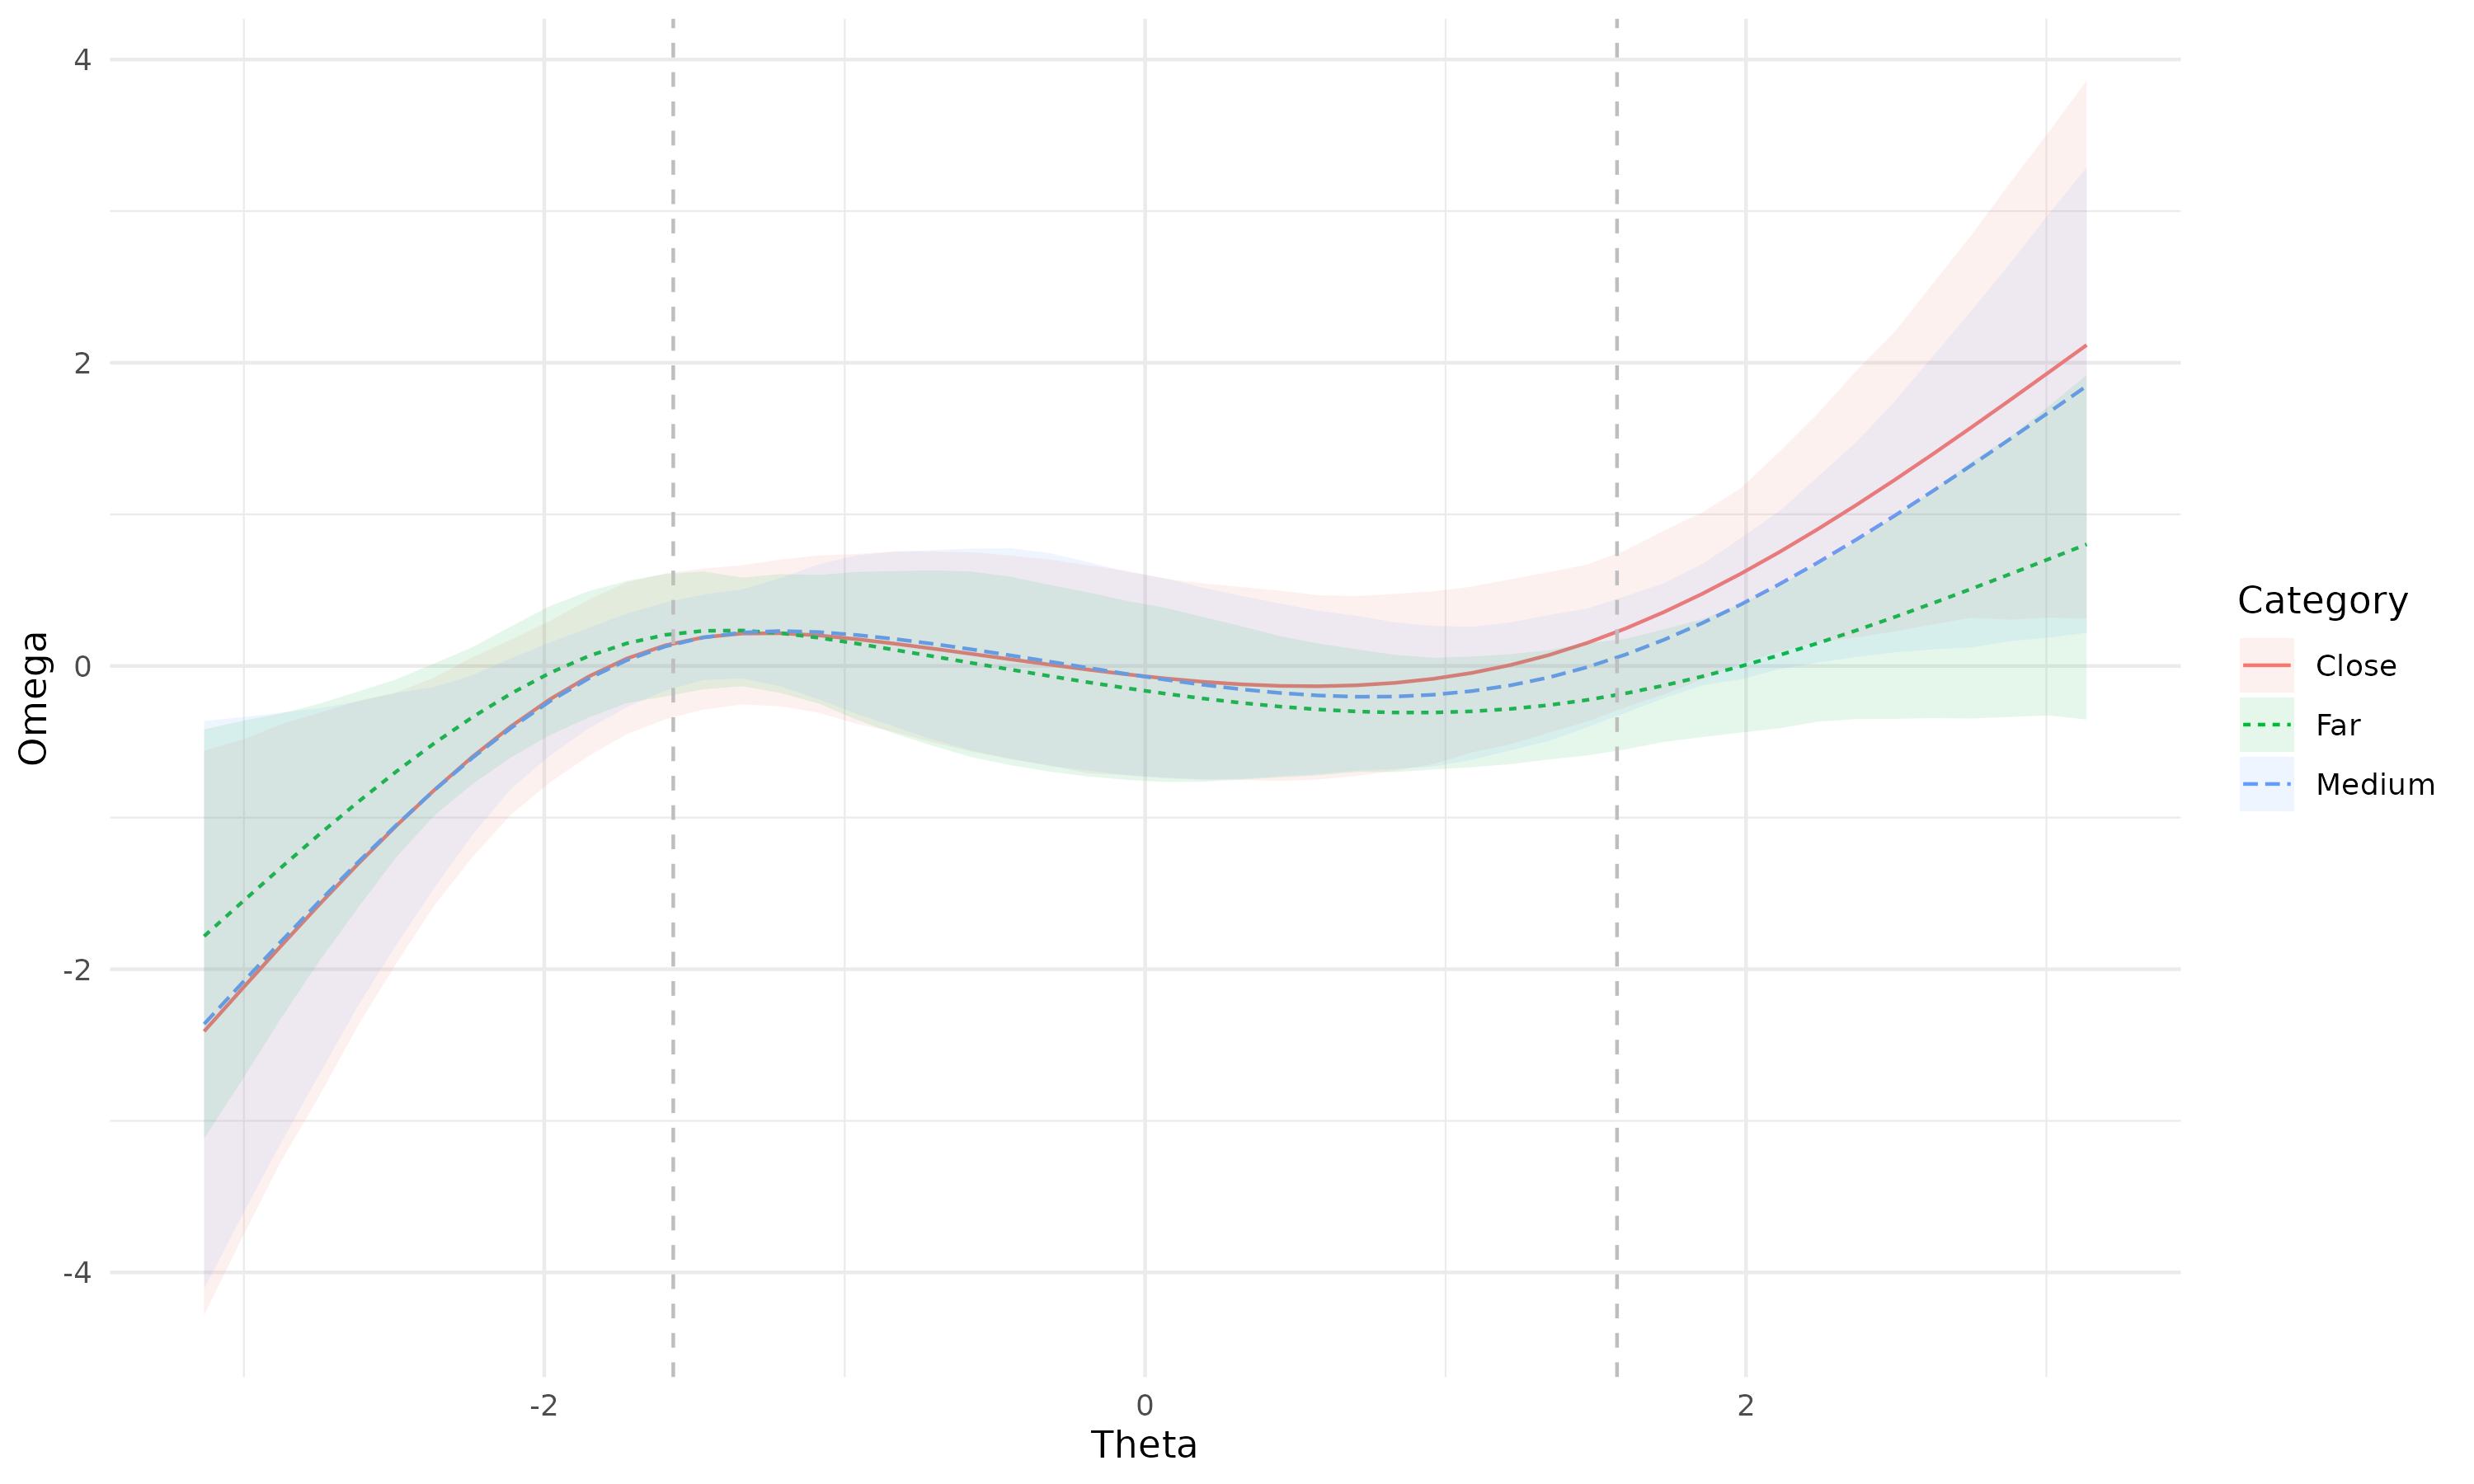
\includegraphics[width=0.7\linewidth]{"images/application/baseline/omega_DistanceShore_levels.pdf"}
	\caption{Estimated smooth $\omega$ as a function of the angle $\Theta$ for fixed distances to the shore: $250$ metres for close, $1.41$ km for medium, and $3$ km or more for far (no effect of the shore).}
	
	\label{fig:febaseline3omegaanglenormalq0}
\end{figure}


Fixing a high standard deviation for the measurement error tends to increase the estimate of the parameter $\tau$. Intuitively, for a low value of the measurement error, a tortuous trajectory can only be caused by less persistent movement, whereas if the measurement error is high, a part of the tortuosity can be attributed to the measurement errors, and therefore a higher estimate of the persistence parameter. We fixed the measurement errors $\sigma_{obs}$ at different values and found that the highest log-likelihood value was obtained for a standard deviation $\sigma_{obs}$ close to $50$m. More details can be found in Appendix.


\subsection{Response estimation}

The baseline estimates of the spline coefficients $\omega_k$, the intercepts $\log(\tau_0)$, $\log(\nu_0)$ and the standard deviations $\sigma_{\tau}$, $\sigma_{\nu}$ are used as offsets in the response model. Only the sound exposure effects on $\tau$ and $\nu$ are estimated from the data after exposure.
Estimates and $95\%$ confidence intervals are shown in Table~\ref{table: response estimations}. As the coefficients $\alpha_\tau$ and $\alpha_\nu$ significatively deviate from zero, this suggests that sound exposure influences both the persistence and the velocity of the movement.\\
%However, we miss the uncertainty coming from the baseline estimates here. To better quantify this uncertainty, we draw $100$ "posterior" samples of the coefficients of the baseline using the Hessian matrix of the log-likelihood to approximate the covariance, and we use the drawn coefficients as offsets for the response model. The mean of the estimates and the standard error over the $100$ estimations are $mean(\hat{\alpha}_\tau)=-3.26$, $mean(\hat{\alpha}_\nu)=0.86$, $mean(\hat{\sigma}_{\alpha_\tau})=0.57$ and $mean(\hat{\sigma}_{\alpha_\nu})=0.27$. \\

\begin{table}[ht!]
	\centering
	\begin{tabular}{|c|c|c|}
		\hline
		Coefficient   & Estimate  & $95 \%$ CI \\
		\hline
		$\alpha_\tau$    & $-3.43$    &  $[-4.77; -2.04]$ \\
		$\alpha_\nu$  & $0.74$   &  $[0.23; 1.25]$\\
		\hline
	\end{tabular}
	\caption{Estimate of the parameters in the log-linear response model}
	\label{table: response estimations}
\end{table}



The estimated $\tau$ and $\nu$ are shown in Figure~\ref{fig: me response} as a function of the distance to the sound source. The value of $\nu$ increases with increased exposure to the sound. This should not come as a surprise since, for instance, the average empirical velocity norm when the narwhals are less than $5$ km away from the ship is $5.7$ km/h, which is more than $1$ km/h higher than the average empirical velocity norm before exposure. 

We draw special attention to the parameter $\tau$, which decreases with increased exposure to the ship, implying lower persistence and lower autocorrelation in the velocity of the narwhals. This had been hinted at in \citep{heide-jorgensen_behavioral_2021}, where it was shown that the narwhals have more tendency to change direction and move towards the shore in presence of the ship. This can be interpreted as a drop in persistence due to the appearance of the ship. Our analysis suggests that the magnitude of this drop might be alarming: for most of the narwhals, at distance less than $5$ km from the ship, the persistence is half the baseline value. This is evidence of a strong shift in the behavior of the whales, which might have consequences on their capacity to rest and forage at short term.


\begin{figure}[ht!]
	\begin{subfigure}{0.98\textwidth}\centering
		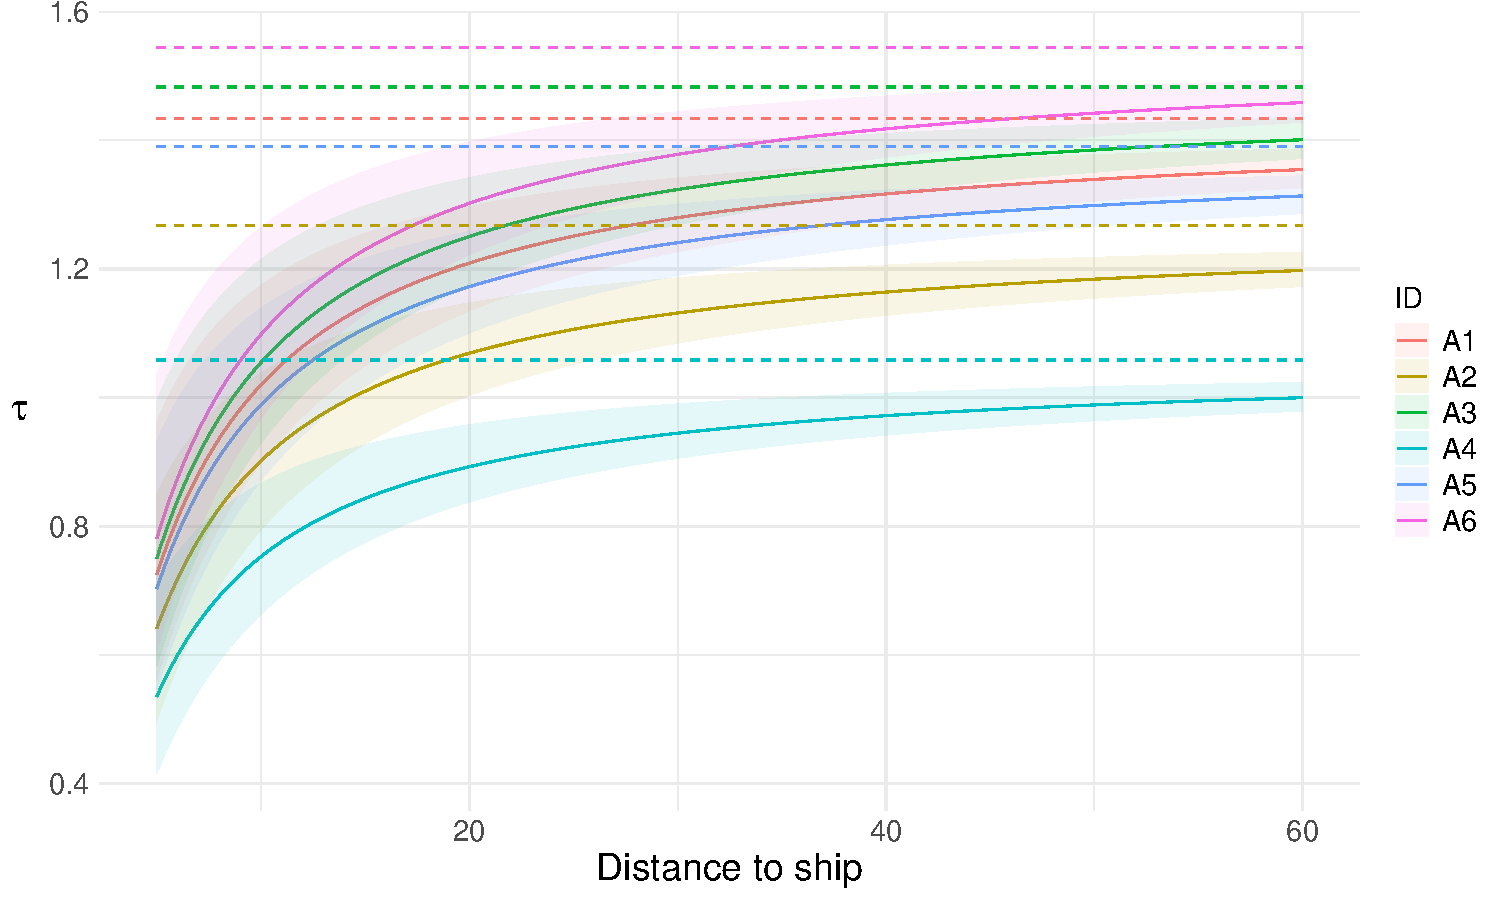
\includegraphics[width=0.7\linewidth]{"images/application/response/plot_me_tau_updated.pdf"}
		\caption{}
	\end{subfigure}
	
	\begin{subfigure}{0.98\textwidth}
		\centering
		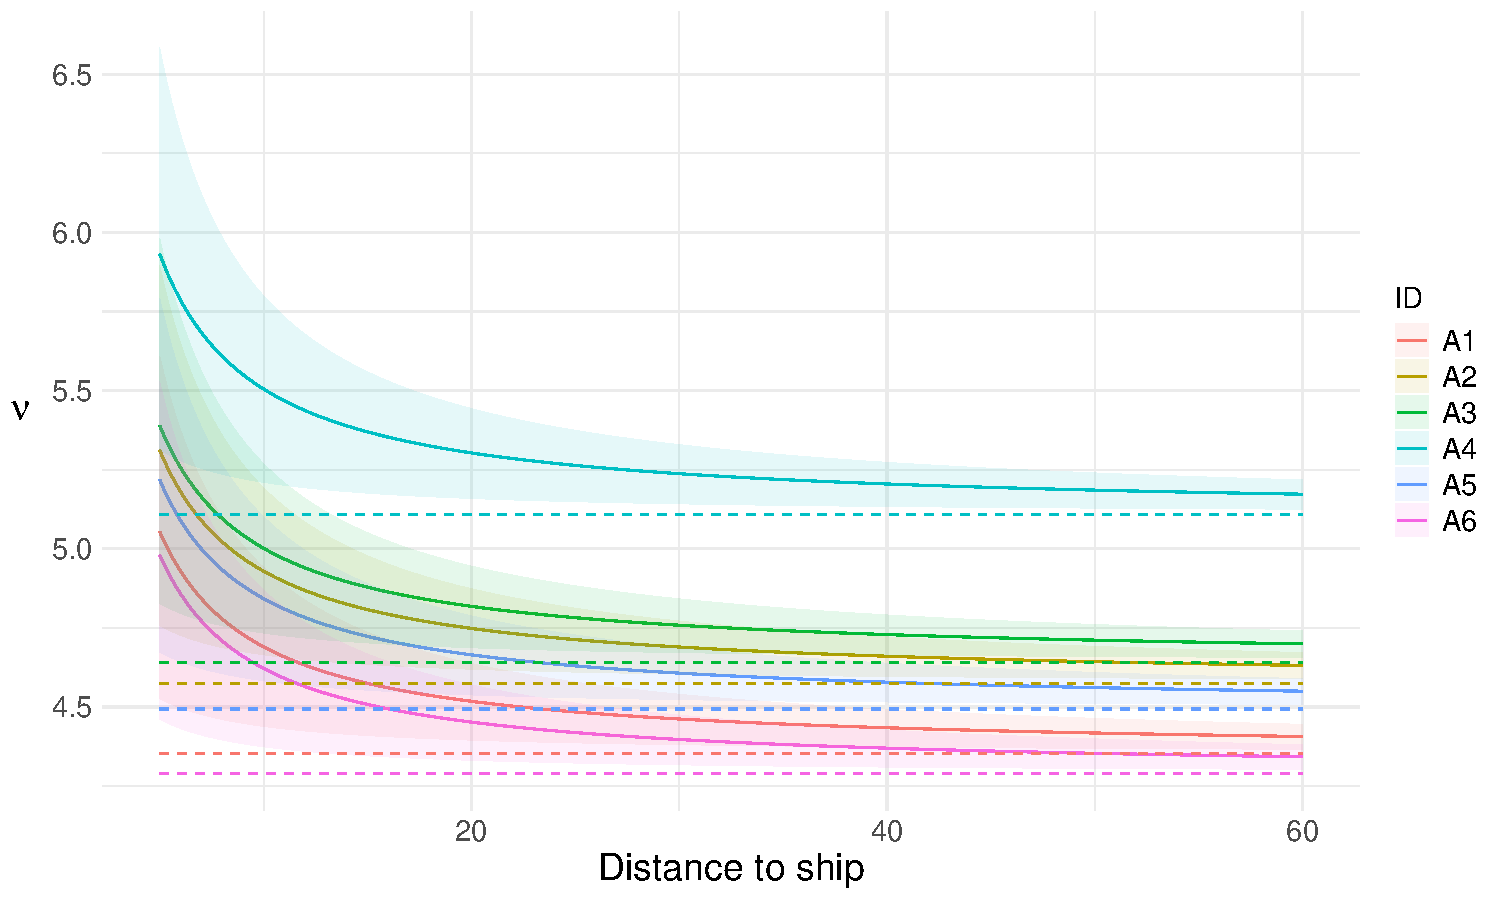
\includegraphics[width=0.7\linewidth]{"images/application/response/plot_me_nu_updated.pdf"}
		\caption{}
	\end{subfigure}
	\caption{Estimated effect of ship exposure on the parameters. The horizontal dashed lines represent the baseline values for each individual. The values on the $x$-axis are in kilometres. (a)  Persistence parameter $\tau$. Values on the $y$-axis are in hour. (b) Velocity parameter $\nu$. Values on the $y$-axis are in km/h.}
	\label{fig: me response}
\end{figure}

The distances to the ship $D^{ship}_{\tau}(p)$ and $D^{ship}_{\nu}(p)$  for which a percentage $p$ of deviation from the population baseline values $\tau_0$ and $\nu_0$ are reached are given by 
\begin{equation}
	D^{ship}_{\tau}(p)=\frac{\alpha_{\tau}}{\log(1-p)} \quad  \mbox{and} \quad  D^{ship}_{\nu}(p)=\frac{\alpha_{\nu}}{\log(1+p)}
\end{equation}
Table~\ref{table: baseline vs response parameters comparison} shows these values for different proportions $p$.
For $\tau$, $90\%$ of the baseline value is recovered at a distance about $32$ km. For $\nu$, $110\%$ of the baseline value is reached at a distance about $7$ km. This indicates that sound exposure can be perceived and can disturb the narwhals motion up to tens of kilometres.


We want to point out that the standard errors for these recovery distances are likely to be underestimated, due to the uncertainty in the baseline estimates, and the dependence between the measurement error and the estimates of the persistence parameters. However, the general take-away remains valid: there is evidence of a decrease in persistence and an increase in velocity up to a couple of tens of kilometers from the sound source. Along with other studies, we believe it can serve as a guideline for mitigation measures towards the effects of anthropogenic noise on the narwhals behavior. 

\renewcommand{\arraystretch}{1.5} % Increase row height by 1.5 times

\begin{table}[ht!]
	\centering
	\begin{tabular}{| c | *{2}{w{c}{4em}|}}
		\hline
		\multirow{2}{*}{Percentage of deviation from baseline} & \multicolumn{2}{c|}{Recovery distance (km) }  \\
		\cline{2-3} 
		& $D^{ship}_{\tau}$ & $D^{ship}_{\nu}$ \\
		\hline
		$50 $ & $4.9 \pm 1.0$ &  $1.8 \pm 0.4$ \\
		$10$ & $32.5 \pm 6.7 $ & $7.8 \pm 2.9$ \\
		\hline
		
	\end{tabular}


	\caption{Estimated recovery distances of the baseline values within a $50 \%$ and $10\%$ range with standard errors.}
	\label{table: baseline vs response parameters comparison}
\end{table}



\section{Conclusion and perspectives}

%summary of the results

We introduced a new method to constrain a stochastic differential equation for animal movement in a bounded region of $\R^2$. Our approach relies on modeling the angular velocity as a function of the distance to the boundary and the angle between the velocity and the boundary normal vector. The additional term that constrains the motion is included in the drift, and, for this reason, acts as a confining potential.
We demonstrated how to simulate such diffusions and how to model different behaviors close to the boundary.\\

This new SDEs with smooth parameters depending on covariates was used to estimate the movement of the narwhals in the fjords. We managed to show an increased tortuosity of the trajectories when approaching the shore. More importantly, we showed that noise exposure has a significant effect on some parameters that drive the motion by comparing a baseline and a response model. We believe this method can be used as a basis for the assessment of behavioral responses in many contexts, and hope it will help understanding better the effects of anthropogenic noise on marine mammals movement.\\

We emphasize that, even if we were able to estimate quite reliably the smooth parameters of the SDE, a part of uncertainty still remains. First, the log-likelihood function that we rely on for the estimation is approximate, based on piecewise constant parameter values on each time step. Given that observations are relatively high frequency (5 min between consecutive observations in median), the error introduced is expected to be low, though we don't have theoretical bounds for it. Moreover, the constant covariate value that is used on each time step is computed from the GPS observations, even though these observations come with GPS measurement error. We don't integrate the measurement error in the covariates $\Theta$, $E^{ship}$ and $I^{shore}$ that we are considering. Since GPS measurement error are pretty low (a few tens of metres) compared to ARGOS for instance, this may not introduce significant error in the estimations. Eventually, Laplace approximation is used to approach the integral of likelihood over the random effects. We did not discuss the error that may be introduced by this approximation, but the simulation study show that despite all the approximations made along the way, we are indeed able to get reliable estimates even for pretty complex models.\\

In the future, studying theoretical properties of the SDE models we used here might be of significant interest. For instance, we did not prove any result or exhibit clear assumptions that would guarantee that the process is effectively constrained. We noticed that in the literature of animal movement modeling, whether that would be with SDEs, HMM or step-selection functions, spatial constraints are rarely considered. We hint that better considerations of the spatial constraints can give new insights into the interactions between marine mammals and their environment.


%%%%%%%%%%%%%%%%%%%%%%%%%%%%%%%%%%%%%%%%%%%%%%
%% Support information, if any,             %%
%% should be provided in the                %%
%% Acknowledgements section.                %%
%%%%%%%%%%%%%%%%%%%%%%%%%%%%%%%%%%%%%%%%%%%%%%


%%%%%%%%%%%%%%%%%%%%%%%%%%%%%%%%%%%%%%%%%%%%%%
%% Funding information, if any,             %%
%% should be provided in the                %%
%% funding section.                         %%
%%%%%%%%%%%%%%%%%%%%%%%%%%%%%%%%%%%%%%%%%%%%%%
\begin{funding}
% The first author was supported by ...
The authors would like to thank the CNRS and IRN Madef for funding A. Delporte, and MIAI - ANR-19-P3IA-0003 for the funding of A Samson.
We also thank the project MATH-AmSud 23-MATH-12.
% The second author was supported in part by ...
\end{funding}

%%%%%%%%%%%%%%%%%%%%%%%%%%%%%%%%%%%%%%%%%%%%%%
%% Supplementary Material, including data   %%
%% sets and code, should be provided in     %%
%% {supplement} environment with title      %%
%% and short description. It cannot be      %%
%% available exclusively as external link.  %%
%% All Supplementary Material must be       %%
%% available to the reader on Project       %%
%% Euclid with the published article.       %%
%%%%%%%%%%%%%%%%%%%%%%%%%%%%%%%%%%%%%%%%%%%%%%
\begin{supplement}
\stitle{Shapefile for land geometry}
\sdescription{Shapefile based on OpenStreetMap data for the land polygons in Scoresby Sound fjords system. We used high resolution satellite images to improve it with \texttt{qgis} software}.
\end{supplement}

%%%%%%%%%%%%%%%%%%%%%%%%%%%%%%%%%%%%%%%%%%%%%%%%%%%%%%%%%%%%%
%%                  The Bibliography                       %%
%%                                                         %%
%%  imsart-nameyear.bst  will be used to                   %%
%%  create a .BBL file for submission.                     %%
%%                                                         %%
%%  Note that the displayed Bibliography will not          %%
%%  necessarily be rendered by Latex exactly as specified  %%
%%  in the online Instructions for Authors.                %%
%%                                                         %%
%%  MR numbers will be added by VTeX.                      %%
%%                                                         %%
%%  Use \citep{...} to cite references in text.             %%
%%                                                         %%
%%%%%%%%%%%%%%%%%%%%%%%%%%%%%%%%%%%%%%%%%%%%%%%%%%%%%%%%%%%%%

\bibliographystyle{imsart-nameyear} % Style BST file
\bibliography{aoas-template}       % Bibliography file (usually '*.bib')
\end{document}
